\documentclass[12pt,english,openany,letterpaper,pagesize]{scrbook}

\usepackage[utf8]{inputenc}
\usepackage[hidelinks]{hyperref}
\usepackage[spanish]{babel}
%\usepackage[spanish]{algorithm2e}
\usepackage{fancyhdr}
\usepackage{epsfig}
\usepackage{epic}
\usepackage{eepic}
\usepackage{amsmath}
\usepackage{threeparttable}
\usepackage{amscd}
\usepackage{here}

\usepackage{algorithm}
\usepackage{algorithmic}
\usepackage{listings}
\usepackage{lscape}
\usepackage{tabularx}
\usepackage{subfigure}
\usepackage{longtable}
\usepackage{nameref}
\usepackage[utf8]{inputenc}
\usepackage{hyperref}
%\usepackage{svg}
\usepackage{cleveref}
\usepackage{siunitx}
\usepackage{gensymb}
\usepackage{eurosym}
\usepackage{multirow}
\usepackage{multicol}
\usepackage{rotating} %Para rotar texto, objetos y tablas seite. No se ve en DVI solo en PS. Seite 328 Hundebuch
                        %se usa junto con \rotate, \sidewidestable ....
\usepackage{graphicx}
\usepackage{siunitx}
 %\usepackage{hyperref} % CAJAS ROJAS
%\usepackage{xcolor}
\usepackage{subfig}

% \usepackage[a4paper, top=2.5cm, bottom=2.5cm, left=2.5cm, right=2.5cm]{geometry}
% \usepackage{graphicx}     % Para \includegraphics
\usepackage{subcaption}   % Para \begin{subfigure}
\usepackage{caption}
\captionsetup{font=small}
\captionsetup[sub]{font=small,skip=2pt}

\usepackage{algorithm}
\usepackage{algpseudocode}
\usepackage{amsmath} % Para símbolos matemáticos

% \usepackage{booktabs}     % Para \toprule, \midrule, \bottomrule
% \usepackage{amsmath}      % Para símbolos matemáticos (como \approx)


\usepackage{longtable} % Paquete para tablas que pueden extenderse en múltiples páginas
\usepackage{caption}   % Para personalizar captions si se desea

\usepackage{subcaption}
\usepackage{booktabs}

\renewcommand{\theequation}{\thechapter-\arabic{equation}}
\renewcommand{\thefigure}{\textbf{\thechapter-\arabic{figure}}}
\renewcommand{\thetable}{\textbf{\thechapter-\arabic{table}}}


\pagestyle{fancyplain}%\addtolength{\headwidth}{\marginparwidth}
\textheight22.5cm \topmargin0cm \textwidth16.5cm
\oddsidemargin0cm \evensidemargin-0cm%
\renewcommand{\chaptermark}[1]{\markboth{\thechapter\; #1}{}}
\renewcommand{\sectionmark}[1]{\markright{\thesection\; #1}}
\lhead[\fancyplain{}{\thepage}]{\fancyplain{}{\rightmark}}
\rhead[\fancyplain{}{\leftmark}]{\fancyplain{}{\thepage}}
\fancyfoot{}
\thispagestyle{fancy}%


\addtolength{\headwidth}{0cm}
\unitlength1mm %Define la unidad LE para Figuras
%\mathindent0cm %Define la distancia de las formulas al texto,  fleqn las descentra
\marginparwidth0cm
\parindent0cm %Define la distancia de la primera linea de un parrafo a la margen

%Para tablas,  redefine el backschlash en tablas donde se define la posici\'{o}n del texto en las
%casillas (con \centering \raggedright o \raggedleft)
\newcommand{\PreserveBackslash}[1]{\let\temp=\\#1\let\\=\temp}
\let\PBS=\PreserveBackslash

%Espacio entre lineas
\renewcommand{\baselinestretch}{1.1}

%Neuer Befehl f\"{u}r die Tabelle Eigenschaften der Aktivkohlen
\newcommand{\arr}[1]{\raisebox{1.5ex}[0cm][0cm]{#1}}

%Neue Kommandos
\usepackage{Befehle}
%Inicio del documento. Tener en cuenta que hay archivos auxiliares

\begin{document}
\pagenumbering{roman}
%\newpage
%\setcounter{page}{1}
\begin{center}
\begin{figure}
\centering%

\epsfig{file=HojaTitulo/LogoUniandes,scale=0.45}%
\end{figure}
\thispagestyle{empty} \vspace*{1.0cm} \textbf{\Large
Sistema de detección de intrusiones para redes IoT mediante TinyML, aprendizaje federado jerárquico y cifrado ligero ASCON-128 en una arquitectura Edge--Fog--Cloud}\\[4.0cm]
\Large\textbf{Santiago Alejandro Jaimes Puerto}\\
\Large\textbf{Nicolas Casas Ibarra}\\[5.0cm]
\small Universidad de Los Andes\\
Departamento de Ingeniería de sistemas y computación\\
Bogotá, Colombia\\
2026\\
\end{center}

\newpage{\pagestyle{empty}\cleardoublepage}

\newpage
\begin{center}
\thispagestyle{empty} \vspace*{0cm} \textbf{\Large Sistema de detección de intrusiones para redes IoT mediante TinyML, aprendizaje federado jerárquico y cifrado ligero ASCON-128 en una arquitectura Edge--Fog--Cloud.}\\[3.0cm]
\Large\textbf{Santiago Alejandro Jaimes Puerto}\\
\Large\textbf{Nicolas Casas Ibarra}\\[3.0cm]
\small University de Los Andes\\
\small Presentado en cumplimiento parcial de los requisitos para el grado de:\\
\textbf{System and Computer engineer}\\[2.0cm]
Director:\\
Prof. Carlos Andrés Lozano Garzón, PhD\\

Trabajo de grado defendido en:\\
Mayo 24, 2026 - 12:00 pm \\[1.5cm]
Universidad de Los Andes\\
Departamento de Ingeniería de Sistemas y Computación\\
Bogotá, Colombia\\
2026\\
\end{center}

\newpage{\pagestyle{empty}\cleardoublepage}

\newpage
\thispagestyle{empty} \textbf{}\normalsize
\\\\\\%
\textbf{Agradecimientos}\\[4.0cm]



        Quiero expresar mi más sincera gratitud a todas las personas que hicieron posible este logro.\\

        A mi familia, quienes han sido mi ancla y mi inspiración en cada paso de este camino. Su amor incondicional y apoyo constante me han dado la fortaleza para superar cualquier desafío. \\
        
        Al profesor Paulo de Oliveria, mi asesor, quien no solo compartió generosamente su conocimiento y experiencia, sino que también fue un guía incansable durante este proyecto. Su paciencia, dedicación y constante disposición para resolver dudas fueron esenciales para enfrentar los retos que surgieron. Sus valiosos comentarios y orientaciones me permitieron aprender y crecer, tanto a nivel académico como personal. Este proyecto no habría sido lo mismo sin su acompañamiento e inspiración. \\

        A la Universidad de los Andes, mi alma máter, por ser un espacio de excelencia académica que me permitió desarrollar mis habilidades y consolidar mi formación profesional. A sus profesores, administrativos y recursos de investigación, les agradezco por fomentar un ambiente de aprendizaje integral, colaboración y crecimiento personal. Haber formado parte de esta comunidad académica ha sido un privilegio invaluable que marcará para siempre mi trayectoria. \\
        
        Y, con un cariño especial, a mis amigos. Gracias por convertir este recorrido en una aventura inolvidable. A Sebastián Moya,  por su apoyo clave y su disposición.\\
        
        A todos ustedes, mi eterno agradecimiento. Este logro también es suyo.
        



\newpage{\pagestyle{empty}\cleardoublepage}




\textbf{\LARGE Resumen}\\

Este documento presenta el diseño, implementación y evaluación de un sistema de detección de intrusiones (IDS) para redes IoT/MQTT desplegado en una arquitectura jerárquica Edge--Fog--Cloud. El sistema combina modelos livianos de \textit{machine learning} ejecutados en microcontroladores ESP32-S3, aprendizaje federado jerárquico (HFL) coordinado desde gateways Raspberry Pi 4 y un servidor PC, y cifrado ligero \textbf{ASCON-128} para proteger el ciclo de aprendizaje. La investigación evalúa cuatro dimensiones: viabilidad de TinyML en el borde, reducción de transferencia de datos mediante HFL, overhead criptográfico de ASCON y comparación entre variantes de arquitectura y modelo.\\

Se diseñó un perceptrón multicapa (MLP) compacto de 1\,139 parámetros ($\approx$4.5\,KB) con arquitectura $13 \to 32 \to 16 \to 8 \to 3$, capaz de clasificar flujos de red en tres categorías (\texttt{normal}, \texttt{mqtt\_bruteforce}, \texttt{scan\_A}) utilizando 13 características extraídas de flujos. El sistema federado comparte únicamente las dos últimas capas del modelo (163 parámetros) y fue evaluado en las ramas \texttt{hfl\_v7-RN}, \texttt{hfl\_v7-no-ascon} y \texttt{hfl\_v7-CNN}, incluyendo modo estándar y modo FOG.\\

Como línea base, se entrenaron modelos clásicos centralizados, alcanzando hasta 99.94\% de accuracy con Random Forest, aunque con requerimientos de memoria incompatibles con microcontroladores. El notebook general de entrenamiento comparó además MLP/RN, CNN-1D, Residual-MLP y Tiny Transformer; el MLP/RN obtuvo el mejor balance entre precisión offline ($\approx$90.6\%), tamaño e implementación en ESP32. La cuantificación del overhead de ASCON-128 mostró costo temporal bajo frente a la duración de las rondas federadas y un incremento moderado del tamaño de los mensajes, sin degradación observable de convergencia.\\

Los resultados validan que la combinación de TinyML, aprendizaje federado y cifrado ligero constituye una solución viable y segura para detección de intrusiones en el borde de redes IoT, ofreciendo un compromiso efectivo entre precisión, privacidad, seguridad y eficiencia computacional.\\


{\small \textbf{Keywords}: Detección de Intrusiones, IoT, TinyML, Aprendizaje Federado Jerárquico, ASCON-128, Criptografía Ligera, Edge--Fog--Cloud, ESP32-S3, Raspberry Pi, CNN-1D, MLP, Seguridad de Redes.}

\renewcommand{\tablename}{\textbf{Table}}
\renewcommand{\figurename}{\textbf{Figure}}
\renewcommand{\listtablename}{Lista de Tablas}
\renewcommand{\listfigurename}{Lista of Figuras}
\renewcommand{\contentsname}{Tabla de Contenido}


%\newcommand{\clearemptydoublepage}{\newpage{\pagestyle{empty}\cleardoublepage}}
\tableofcontents

\clearpage

\addcontentsline{toc}{chapter}{List of Figures} % para que aparezca en el indice de contenidos
\listoffigures % indice de figuras

\clearpage
\addcontentsline{toc}{chapter}{List of Tables} % para que aparezca en el indice de contenidos
\listoftables % indice de tablas

\clearpage
%\input{Tab_Simbolos/TabSimbolosMSc}
%\input{Resumen}%\newcommand{\clearemptydoublepage}{\newpage{\pagestyle{empty}\cleardoublepage}}
\pagenumbering{arabic}
\chapter{Introducción}
\label{chap:Introduction}

\section{Contexto}

La adopción de redes \textit{Internet of Things} (IoT) e \textit{Industrial IoT} (IIoT) ha aumentado la superficie de ataque de hogares, laboratorios, plantas industriales y sistemas de monitoreo conectados. Estos entornos combinan dispositivos heterogéneos, protocolos livianos como MQTT, conectividad intermitente y capacidades limitadas de cómputo, lo que dificulta desplegar mecanismos de detección convencionales basados en procesamiento centralizado. Bajo marcos de gestión de riesgo como el \textit{NIST Cybersecurity Framework}, la detección temprana y el monitoreo continuo son capacidades fundamentales para reducir el tiempo de respuesta ante incidentes \cite{NISTCSF2024}.

Los sistemas de detección de intrusiones de red (NIDS) basados en aprendizaje automático han mostrado altos niveles de precisión en condiciones de laboratorio. Sin embargo, muchos de estos resultados se obtienen bajo supuestos que no siempre se cumplen en IoT: centralización de datos, disponibilidad de servidores con alta memoria, ausencia de cifrado en las comunicaciones internas del sistema y modelos demasiado grandes para ejecutarse en microcontroladores. En consecuencia, el reto no consiste únicamente en maximizar \textit{accuracy}, sino en validar una arquitectura completa que pueda operar sobre hardware restringido, actualizarse de manera distribuida y proteger los artefactos del aprendizaje.

Esta tesis aborda ese reto mediante una arquitectura Edge--Fog--Cloud para detección de intrusiones en tráfico MQTT. La capa Edge se implementa con nodos ESP32-S3 que ejecutan inferencia TinyML y transmiten características de flujo; la capa Fog se implementa sobre Raspberry Pi 4 como gateway MQTT, entrenador local y agregador intermedio; y la capa Cloud se implementa en un PC con FastAPI para coordinar la agregación global. El sistema se evaluó en varias configuraciones de la versión \texttt{hfl\_v7}: red neuronal MLP con ASCON-128, red neuronal MLP sin ASCON como línea base, variante CNN-1D y estrategia FOG con agregación entre gateways.

\section{Problemática}

La primera brecha identificada es la \textbf{viabilidad de despliegue}. Modelos centralizados como Random Forest o SVM-RBF pueden alcanzar precisiones cercanas al 100\%, pero sus requerimientos de memoria son incompatibles con microcontroladores. En contraste, un IDS IoT real necesita inferencia frecuente, bajo consumo de memoria y comunicación limitada.

La segunda brecha corresponde a la \textbf{privacidad y distribución de datos}. Centralizar capturas PCAP o flujos completos desde múltiples redes introduce costos de transferencia y riesgos de exposición. El aprendizaje federado reduce este problema al compartir pesos o gradientes en lugar de datos crudos, pero en IoT introduce retos adicionales: datos \textit{non-IID}, rondas incompletas, heterogeneidad de hardware y sobrecarga de comunicación \cite{Imteaj2022_FL_ResourceConstrainedSurvey, Albanbay2025}.

La tercera brecha es la \textbf{seguridad del propio ciclo federado}. Aunque FL evita mover datos crudos, los pesos del modelo, métricas locales y mensajes de control siguen siendo activos sensibles. Por tanto, las comunicaciones entre ESP32, Raspberry Pi y PC deben proteger confidencialidad e integridad con mecanismos compatibles con dispositivos restringidos. ASCON-128, estandarizado por NIST como criptografía ligera, es una opción pertinente para este escenario \cite{NISTSP8002322025}.

Finalmente, el sistema debe ser evaluado como arquitectura, no solo como modelo. Por eso se comparan cuatro dimensiones: desempeño del modelo TinyML, costo del aprendizaje federado, overhead de ASCON-128 y efecto de variar el modelo o la topología mediante las ramas \texttt{hfl\_v7-RN}, \texttt{hfl\_v7-no-ascon} y \texttt{hfl\_v7-CNN}.

\section{Justificación}

La solución propuesta aporta una validación práctica de un IDS federado para IoT sobre hardware real. A diferencia de un entrenamiento centralizado, el sistema opera con un modelo compacto de 13 características de flujo y tres clases de tráfico: \texttt{normal}, \texttt{mqtt\_bruteforce} y \texttt{scan\_A}. Este alcance permite instrumentar el ciclo completo de detección, entrenamiento local, agregación global y redistribución del modelo sin depender de infraestructura de alto costo en el borde.

El proyecto también justifica la comparación entre variantes. La rama con ASCON-128 permite medir el costo de proteger todos los canales; la rama sin ASCON sirve como línea base para aislar el overhead criptográfico; la variante CNN-1D evalúa si una arquitectura más expresiva mejora el desempeño sin romper la viabilidad edge; y el modo FOG introduce una agregación intermedia entre Raspberry Pi antes del servidor central.

El componente de NLP sobre logs, considerado en objetivos tempranos del proyecto, no forma parte del despliegue final de \texttt{hfl\_v7}. En esta versión se deja como línea futura, mientras que el aporte implementado se concentra en características numéricas de flujo, TinyML, HFL y cifrado ligero. Esta delimitación es importante para mantener consistencia entre código, resultados y conclusiones.

El documento está estructurado de la siguiente manera: el Capítulo~\ref{chap:Introduction} presenta el problema y los objetivos; el Capítulo~\ref{chap:theo} resume el marco conceptual y el estado del arte; el Capítulo~\ref{chap:meth} describe la arquitectura y el protocolo experimental; el Capítulo~\ref{chap:resu} presenta resultados; el Capítulo~\ref{chap:conc} concluye y plantea trabajos futuros; y los anexos resumen archivos y artefactos del sistema.

\section{Objetivos}

\subsection{Objetivo General}
Diseñar, implementar y evaluar un sistema de detección de intrusiones para tráfico IoT/MQTT basado en TinyML, aprendizaje federado jerárquico y cifrado ligero ASCON-128, desplegado sobre una arquitectura Edge--Fog--Cloud compuesta por ESP32-S3, Raspberry Pi 4 y un servidor PC.

\subsection{Objetivos Específicos}
\begin{enumerate}
    \item Construir un \textit{pipeline} de datos basado en flujos de red unidireccionales, seleccionando 13 características computables en dispositivos de borde y definiendo un problema triclase para tráfico \texttt{normal}, \texttt{mqtt\_bruteforce} y \texttt{scan\_A}.

    \item Entrenar y comparar modelos compactos para IDS IoT, incluyendo MLP, CNN-1D, Residual-MLP y Tiny Transformer, exportando pesos y parámetros de normalización para ejecución en ESP32-S3.

    \item Implementar una arquitectura HFL bidireccional donde los gateways Raspberry Pi entrenan localmente, envían pesos al servidor central, reciben el modelo global y lo redistribuyen a los nodos ESP32.

    \item Evaluar el impacto del cifrado ASCON-128 frente a una línea base sin cifrado, midiendo tiempo de cifrado/descifrado, tamaño de mensajes y efecto sobre la convergencia del modelo.

    \item Analizar el efecto de variar la arquitectura del modelo y la topología de agregación mediante las ramas \texttt{hfl\_v7-RN}, \texttt{hfl\_v7-no-ascon}, \texttt{hfl\_v7-CNN} y el modo FOG.
\end{enumerate}

\subsection{Preguntas de investigación}
\begin{enumerate}
    \item ¿Puede un modelo TinyML ejecutado en ESP32-S3 detectar tráfico MQTT malicioso con precisión operativamente viable?
    \item ¿Qué reducción de transferencia de datos se obtiene al usar HFL en lugar de centralizar los flujos de red?
    \item ¿Cuál es el costo temporal y de comunicación de proteger el ciclo federado con ASCON-128?
    \item ¿Cómo cambian los resultados al comparar MLP, CNN-1D, baseline sin ASCON y agregación FOG?
\end{enumerate}

\chapter{Marco Teórico}
\label{chap:theo}

\section{Marco Conceptual}
\label{sec:conceptos}

\subsection{IDS en redes IoT/IIoT}
Un sistema de detección de intrusiones de red (NIDS) monitorea tráfico y eventos para identificar comportamientos maliciosos o anómalos. En IoT/IIoT, esta tarea es más exigente que en redes tradicionales porque los dispositivos tienen recursos limitados, usan protocolos livianos, presentan patrones de tráfico heterogéneos y suelen estar distribuidos en dominios administrativos distintos. Por ello, la detección debe evaluarse no solo por \textit{accuracy}, sino también por latencia, memoria, comunicación y estabilidad operacional \cite{Tekin2023_OnDeviceEnergy, Amuthadevi2025}. Surveys recientes sobre seguridad IIoT habilitada por ML insisten en que la diversidad de capas (sensor, gateway, fog, cloud) impide soluciones monolíticas y favorece arquitecturas jerárquicas con responsabilidades repartidas \cite{Ni2024_IIoT_Security_Survey, Amanullah2020_DL_BigData_IoT_Security}. Frameworks anteriores combinaron SDN/NFV con ML para coordinar respuesta y monitoreo (\emph{e.g.,}\cite{Bagaa2020_ML_IoT_Framework, Huda2018_DBN_SCADA}), e incluso frameworks ML basados en cloud para gestionar la seguridad de IoT~\cite{Mohamed2024_ML_CloudIoT}, pero rara vez mostraron despliegue sobre microcontroladores reales.

\subsection{Representación por flujos}
El tráfico de red puede representarse como paquetes, capturas PCAP, logs o flujos. Esta tesis utiliza flujos unidireccionales porque son compactos, tabulares y computables en el borde. Cada flujo se transforma en 13 características numéricas relacionadas con conteo de paquetes, tiempos entre paquetes, tamaños de paquetes, bytes totales y banderas TCP. Esta representación sacrifica parte del detalle secuencial de un PCAP completo, pero permite inferencia TinyML en ESP32-S3 y reduce el volumen de comunicación.

\subsection{TinyML y modelos compactos}
TinyML agrupa técnicas para ejecutar modelos de aprendizaje automático en hardware restringido. En el contexto de esta tesis, el criterio de diseño es que el modelo pueda ejecutarse directamente en microcontroladores ESP32-S3 sin depender de aceleradores externos ni transferir los datos crudos al servidor. La revisión de Dini~\textit{et~al.}~\cite{Dini2024_EmbeddedIIoT_Review} resume el ecosistema actual de \emph{toolchains} (TensorFlow Lite Micro, STM32Cube.AI, Vitis~AI, etc.) y muestra que la integración exitosa depende tanto de la arquitectura del modelo como del soporte HW/SW del MCU. Ficco~\textit{et~al.}~\cite{Ficco2024_FL_TinyML_Onboard} demostraron que el entrenamiento on-board en dispositivos como ESP32 y Arduino MKR1010 es viable cuando se combina FL con \emph{transfer learning}, alcanzando accuracy comparable al entrenamiento centralizado (86.48\% en clasificación) con latencia y consumo controlados. Los modelos evaluados en esta tesis incluyen MLP, CNN-1D, Residual-MLP y Tiny Transformer; sin embargo, el despliegue principal utiliza un MLP compacto por su equilibrio entre tamaño, precisión y simplicidad de inferencia, en línea con las recomendaciones de la literatura para clasificación tabular en MCUs \cite{HeydariMahmoud2025_TinyML_IDS, Dini2024_EmbeddedIIoT_Review}.

\subsection{Aprendizaje federado jerárquico}
El aprendizaje federado (FL) permite entrenar modelos de forma distribuida compartiendo actualizaciones en lugar de datos crudos. En escenarios IoT, una arquitectura jerárquica (HFL) resulta natural porque los nodos edge pueden comunicarse con gateways cercanos y estos, a su vez, con un coordinador central. Este diseño reduce exposición de datos, organiza la comunicación por capas y permite agregar actualizaciones localmente antes de enviarlas al servidor global \cite{McMahan2017FedAvg, Imteaj2022_FL_ResourceConstrainedSurvey}. Hajj~\textit{et~al.}~\cite{Hajj2023_CrossLayerFL_IDS} muestran que un IDS federado \emph{cross-layer} para IoT puede alcanzar precisión competitiva con menor consumo de comunicación, y Chaurasia~\textit{et~al.}~\cite{Chaurasia2024_FL_ResNet_IIoT} evidencian beneficios al usar redes residuales como base del cliente FL en IIoT.

La literatura advierte que FL en IoT enfrenta datos \textit{non-IID}, conectividad irregular y heterogeneidad de hardware \cite{Albanbay2025, Ramadan2025}. En esta tesis, esas condiciones se reproducen parcialmente mediante nodos con distribuciones distintas: un nodo genera tráfico normal y otro genera una mezcla de tráfico normal, fuerza bruta MQTT y escaneo. Adicionalmente, Tran~\textit{et~al.}~\cite{Tran2026_EdgeTrustShard} cuantifican una brecha de memoria de hasta tres órdenes de magnitud entre los métodos de agregación bizantino-resilientes (512\,MB--2\,GB) y los MCU comerciales ($\sim$264\,KB de SRAM), evidenciando la necesidad de descomponer el problema en capas. La arquitectura de esta tesis adopta esa filosofía sin requerir blockchain ni consenso PoP, dejando la robustez bizantina como trabajo futuro.

\subsection{Cifrado ligero y ASCON-128}
Aunque FL reduce la centralización de datos, los pesos del modelo y mensajes de control siguen siendo sensibles. Un atacante que intercepte o modifique actualizaciones podría inferir información, degradar el modelo o introducir comportamiento malicioso. Por esta razón, la arquitectura integra ASCON-128 como cifrado autenticado ligero para proteger confidencialidad e integridad en los canales MQTT y HTTP del ciclo federado.

ASCON fue seleccionado por NIST en febrero de 2023 como estándar de criptografía ligera, después de un proceso multi-anual frente a candidatos como GIFT-COFB, Sparkle, Romulus y TinyJambu \cite{NISTSP8002322025, Kaur2025_ASCON_Survey}. Internamente, ASCON aplica una permutación de 320 bits estructurada en cinco palabras de 64 bits, con dos variantes principales: ASCON-128 (rate 64 bits) y ASCON-128a (rate 128 bits). El survey de Kaur~\textit{et~al.}~\cite{Kaur2025_ASCON_Survey} resume implementaciones FPGA/ASIC, ataques diferenciales, ataques de canal lateral y contramedidas, ofreciendo una guía consolidada para diseñadores de sistemas embebidos. Su diseño resulta apropiado para mensajes pequeños como features, pesos parciales y modelos globales \cite{NISTSP8002322025, Gusita2025_LWC_Survey}.

Una alternativa frecuente en la industria son los protocolos \emph{ultra-lightweight} basados en permutaciones \emph{ad-hoc} (XOR, rotaciones, shifts), pero Mirzaali~\textit{et~al.}~\cite{Mirzaali2025_LWC_Permutations} demuestran experimentalmente sobre tres Raspberry Pi que estos esquemas suelen ser vulnerables a ataques de divulgación completa de secretos y desincronización, incluso cuando la estructura del protocolo parece sólida. Esto refuerza la decisión de usar un AEAD estandarizado en lugar de criptografía hecha en casa. En esta tesis se mide explícitamente su overhead frente a una versión funcionalmente equivalente sin cifrado, replicando el patrón experimental de varios trabajos previos sobre Edge--Cloud con cifrado por atributos \cite{SaravanaBalaji2023_EdgeIoT_DL}.

\subsection{Agregación FOG}
El modo FOG extiende la arquitectura estándar con comunicación entre gateways Raspberry Pi. Un gateway líder recibe actualizaciones de gateways pares mediante MQTT, realiza un FedAvg intermedio y envía al servidor central una actualización preagregada. Este esquema aproxima escenarios reales con múltiples zonas o sedes, donde una capa fog reduce tráfico hacia la nube y permite coordinación local antes de la agregación global. Wang~\textit{et~al.}~\cite{Wang2019_DataFusion_CPSS} discuten cómo la fusión de datos en sistemas ciber-físico-sociales se beneficia de pre-agregación cercana a la fuente, y EdgeTrust-Shard~\cite{Tran2026_EdgeTrustShard} demuestra que distribuir complejidad computacional por la topología es indispensable cuando los participantes son MCUs. El presente trabajo opera en una jerarquía de tres niveles (PC, Pi, ESP32) que materializa esa idea sin introducir blockchain.

\section{Estado del Arte}
\label{sec:antecedentes}

La literatura revisada se agrupa en cuatro líneas, articuladas alrededor de las cuatro dimensiones del sistema (Edge, Fog/FL, criptografía y datasets/etiquetado).

\subsection{IDS y TinyML para IoT/IIoT}
La primera línea aborda IDS para IoT/IIoT y destaca que los modelos de alta precisión no siempre son desplegables en el borde. Trabajos recientes sobre TinyML e IDS enfatizan que la memoria, la latencia y el costo energético deben reportarse junto con las métricas de clasificación \cite{Tekin2023_OnDeviceEnergy, Alwaisi2024, Amuthadevi2025, HeydariMahmoud2025_TinyML_IDS}. Surveys más generales sobre IIoT, DL y big data en seguridad IoT \cite{Amanullah2020_DL_BigData_IoT_Security, Ni2024_IIoT_Security_Survey} muestran que la mayoría de los pipelines reportados se apoyan en servidores capaces y carecen de despliegue real en MCUs. La revisión de Dini~\textit{et~al.}~\cite{Dini2024_EmbeddedIIoT_Review} compila explícitamente la oferta de \emph{toolchains} TinyML (TFLM, STM32Cube.AI, Vitis~AI) y los compromisos al integrarlos en plataformas embebidas.

\subsection{Aprendizaje federado para seguridad IoT}
La segunda línea corresponde al aprendizaje federado aplicado a seguridad IoT. FL permite entrenar modelos sin centralizar datos, pero introduce retos de comunicación, datos \textit{non-IID} y participación parcial. Estudios recientes sobre FL para IDS muestran que la precisión puede degradarse frente al entrenamiento centralizado, pero que la reducción de datos compartidos puede justificar el intercambio en escenarios con restricciones de privacidad \cite{Imteaj2022_FL_ResourceConstrainedSurvey, Albanbay2025, Hajj2023_CrossLayerFL_IDS, Roy2023_FL_AdaptedModel}. Chaurasia~\textit{et~al.}~\cite{Chaurasia2024_FL_ResNet_IIoT} usan redes residuales como cliente FL en IIoT, mientras que Ficco~\textit{et~al.}~\cite{Ficco2024_FL_TinyML_Onboard} validan FL+TL para entrenamiento on-board en MCUs y Raspberry Pi~3, comparando contra TFLite. EdgeTrust-Shard~\cite{Tran2026_EdgeTrustShard} aporta una visión más reciente: cuando los participantes son MCUs, las defensas Byzantine-robust convencionales (Krum, FLTrust, Fed-NGA) son inalcanzables sin descomponer el problema en una jerarquía como la propuesta en este trabajo.

\subsection{Criptografía ligera y autenticación}
La tercera línea es criptografía ligera. ASCON y otros esquemas de bajo costo buscan proteger dispositivos restringidos sin introducir overhead prohibitivo. Para un IDS federado, esta línea es especialmente relevante porque las actualizaciones de modelo son parte del activo de seguridad y deben protegerse durante el tránsito \cite{NISTSP8002322025, Gusita2025_LWC_Survey, Kaur2025_ASCON_Survey}. El survey de Kaur~\textit{et~al.}~\cite{Kaur2025_ASCON_Survey} provee una taxonomía de implementaciones FPGA/ASIC, ataques (diferenciales, cube, fault injection, side-channel) y contramedidas, lo que orienta decisiones de diseño y trabajos futuros. En contraste, Mirzaali~\textit{et~al.}~\cite{Mirzaali2025_LWC_Permutations} muestran cómo permutaciones ultra-ligeras \emph{ad-hoc} para autenticación RFID/IoT se rompen experimentalmente en hardware (RPi + Wi-Fi). Mecanismos complementarios de control de acceso \cite{Amoon2020_RRAC_IoT} y cifrado por atributos \cite{SaravanaBalaji2023_EdgeIoT_DL} se han propuesto para escenarios sanitarios y de smart cities, pero ninguno integra cifrado y FL sobre la misma plataforma.

\subsection{Datasets y representación del tráfico}
La cuarta línea cubre datasets y representación de tráfico. UNSW-NB15, Bot-IoT, TON\_IoT, Edge-IIoTset, IoT-23 y CICIoT2023 \cite{Moustafa2020_TONIoT, UNSW_UNSWNB15_Download, UNSW_BotIoT_Download, UNSW_TONIoT_Download, Ferrag2022_EdgeIIoTset, Stratosphere_IoT23, Neto2023_CICIoT2023} ofrecen capturas etiquetadas con diversos protocolos y vectores de ataque. Trabajos recientes \cite{Rani2024_IoT_IDS_Datasets, Raminenei2023_ML_IoT_UNSWNB15} proponen consolidar/integrar varios datasets para evitar sobreajuste a una sola fuente. En esta tesis se trabaja con tres datasets de flujos unidireccionales (\texttt{normal}, \texttt{mqtt\_bruteforce}, \texttt{scan\_A}) representativos del tráfico que un nodo MQTT puede observar en un laboratorio o smart home.

\section{Síntesis de la Brecha}

Los trabajos existentes suelen cubrir por separado TinyML, FL o cifrado ligero. La brecha abordada en esta tesis es la integración y medición de un ciclo completo Edge--Fog--Cloud sobre hardware real, con inferencia en ESP32-S3, entrenamiento local en Raspberry Pi, agregación global en PC, protección ASCON-128, línea base sin cifrado, variante CNN y modo FOG. Esta evaluación conjunta permite discutir el sistema como una arquitectura operativa y no solo como un clasificador aislado. Cuatro contribuciones específicas distinguen este trabajo:
\begin{enumerate}
    \item Implementación interoperable de ASCON-128 en C++ (ESP32) y Python (RPi/PC), instrumentada con métricas de tiempo y tamaño por canal y por ronda.
    \item Comparación experimental directa, sobre el mismo hardware y mismas condiciones, entre la rama con ASCON y la rama sin ASCON.
    \item Comparación de dos familias de modelos federables (MLP/RN y CNN-1D) bajo el mismo protocolo HFL, con un Tiny Transformer y un Residual MLP como referencias offline.
    \item Estrategia FOG con agregación intermedia entre gateways Raspberry Pi (líder/peer), que no aparece reportada de forma combinada con ASCON-128 en la literatura revisada.
\end{enumerate}

\begin{longtable}{@{}p{0.18\textwidth} p{0.32\textwidth} p{0.42\textwidth}@{}}
\caption{Relación entre literatura y decisiones de diseño.}
\label{tab:literatura_diseno}\\
\toprule
\textbf{Línea} & \textbf{Referencias} & \textbf{Uso en la tesis} \\
\midrule
\endfirsthead
\toprule
\textbf{Línea} & \textbf{Referencias} & \textbf{Uso en la tesis} \\
\midrule
\endhead
TinyML / IDS IoT & \cite{Tekin2023_OnDeviceEnergy, Amuthadevi2025, Alwaisi2024, HeydariMahmoud2025_TinyML_IDS, Dini2024_EmbeddedIIoT_Review} & Selección de modelos compactos, reporte de huella de memoria, latencia de inferencia en ESP32-S3 y elección de \emph{toolchain} de despliegue. \\
Surveys IoT/IIoT seguridad & \cite{Amanullah2020_DL_BigData_IoT_Security, Ni2024_IIoT_Security_Survey, Bagaa2020_ML_IoT_Framework, Huda2018_DBN_SCADA} & Encuadre del problema, justificación de jerarquía Edge--Fog--Cloud y comparación contra enfoques no edge. \\
FL / HFL para IDS & \cite{McMahan2017FedAvg, Imteaj2022_FL_ResourceConstrainedSurvey, Albanbay2025, Ramadan2025, Hajj2023_CrossLayerFL_IDS, Roy2023_FL_AdaptedModel, Chaurasia2024_FL_ResNet_IIoT, Ficco2024_FL_TinyML_Onboard} & Diseño de FedAvg jerárquico, discusión de datos \textit{non-IID} y sustento del entrenamiento on-board en MCUs/RPi. \\
Robustez/escalabilidad FL en MCUs & \cite{Tran2026_EdgeTrustShard} & Justificación de la jerarquía y delimitación de las amenazas no cubiertas (clientes bizantinos). \\
Criptografía ligera & \cite{NISTSP8002322025, Gusita2025_LWC_Survey, Kaur2025_ASCON_Survey, Mirzaali2025_LWC_Permutations, NISTIR8454_2023} & Integración de ASCON-128, comparación contra baseline sin cifrado, justificación de no usar permutaciones \emph{ad-hoc} y delimitación de canales laterales como trabajo futuro. \\
Datasets IoT-IDS & \cite{Moustafa2020_TONIoT, Neto2023_CICIoT2023, Ferrag2022_EdgeIIoTset, Stratosphere_IoT23, Rani2024_IoT_IDS_Datasets, Raminenei2023_ML_IoT_UNSWNB15} & Selección de las 13 features de flujo y de las tres clases (\texttt{normal}, \texttt{mqtt\_bruteforce}, \texttt{scan\_A}). \\
Pre-agregación / data fusion & \cite{Wang2019_DataFusion_CPSS} & Justificación conceptual del modo FOG (FedAvg de gateways antes del PC). \\
\bottomrule
\end{longtable}

\newpage

\chapter{Metodología}
\label{chap:meth}

La presente investigación sigue un enfoque experimental y cuantitativo, estructurado en seis fases: (i) construcción del pipeline de datos, (ii) entrenamiento y comparación offline de modelos livianos, (iii) implementación de la arquitectura jerárquica de aprendizaje federado, (iv) integración de cifrado ligero ASCON-128, (v) construcción de una línea base sin cifrado y (vi) evaluación de variantes con MLP/RN, CNN-1D y estrategia FOG sobre hardware real.

% ====================================================================
\section{Modelo de Amenazas y Suposiciones}
\label{sec:threat_model}

Antes de detallar la arquitectura, se hace explícito el modelo de amenazas que motiva las decisiones de diseño. Se asume un atacante de red pasivo o activo capaz de observar y modificar el tráfico inalámbrico entre nodos ESP32, gateways Raspberry Pi y el PC coordinador, pero \emph{externo} al sistema. Las amenazas que el sistema busca mitigar son:

\begin{itemize}
    \item \textbf{Confidencialidad de pesos y features:} Un atacante que capture los mensajes MQTT/HTTP no debe poder leer el contenido (pesos federados, métricas locales, vectores de features). Esto se garantiza con ASCON-128 sobre todos los canales \cite{NISTSP8002322025, Kaur2025_ASCON_Survey}.
    \item \textbf{Integridad y autenticidad:} Mensajes alterados o inyectados deben ser detectados y descartados. Se usa el tag de autenticación de 128 bits que ASCON-128 produce de forma nativa, evitando el patrón frecuente de combinar cifrado simétrico con HMAC externo \cite{NISTIR8454_2023}.
    \item \textbf{Reuso de mensajes (replay):} Cada nonce se construye a partir de un timestamp truncado a 32 bits y un contador monótono local; combinado con el tag autenticado, esto detecta reutilizaciones aunque un atacante reenvíe un mensaje válido.
    \item \textbf{Diseños criptográficos no estandarizados:} Se descarta el uso de permutaciones ultra-ligeras \emph{ad-hoc} para autenticación, dado que análisis recientes han demostrado vulnerabilidades estructurales explotables sobre Raspberry Pi en condiciones realistas \cite{Mirzaali2025_LWC_Permutations}.
\end{itemize}

\noindent\textbf{Amenazas fuera del alcance.} Se delimitan explícitamente las siguientes amenazas que \emph{no} se mitigan en esta versión del sistema:

\begin{itemize}
    \item \textbf{Clientes bizantinos / data poisoning:} Un gateway o nodo edge comprometido podría enviar pesos manipulados que sesguen el modelo global. La literatura reporta que un 10\% de participantes maliciosos puede degradar la accuracy global de 96\% a 23\% \cite{Tran2026_EdgeTrustShard}. Mitigaciones (Krum, FLTrust, Fed-NGA, MF-PoP) requieren capacidades de cómputo y memoria que exceden las de un MCU sin descomposición arquitectónica adicional. Esta línea queda como trabajo futuro.
    \item \textbf{Ataques de canal lateral sobre ASCON:} Análisis de potencia, EM o fault injection contra la implementación ASCON pueden recuperar la clave si el atacante tiene acceso físico al MCU \cite{Kaur2025_ASCON_Survey}. El sistema asume despliegue en un entorno físico controlado.
    \item \textbf{Inferencia de membresía:} Aunque FL no comparte datos crudos, los pesos pueden filtrar información sobre los datos locales. Defensas como differential privacy (DP-SGD) no se aplican en esta versión.
    \item \textbf{Compromiso del PC coordinador:} El PC se asume confiable (TCB). Trabajos basados en blockchain o multi-coordinador podrían eliminar este supuesto \cite{Tran2026_EdgeTrustShard}.
\end{itemize}


% ====================================================================
\section{Arquitectura del Sistema}
\label{sec:arquitectura}

El sistema propuesto se organiza en tres capas jerárquicas que reflejan la topología Edge--Fog--Cloud, cada una con roles diferenciados de procesamiento, entrenamiento y coordinación.

\subsection{Capa Edge: Nodos ESP32-S3}

Los nodos de borde se implementan sobre microcontroladores \textbf{ESP32-S3} con conectividad Wi-Fi nativa. Cada nodo cumple tres funciones:
\begin{enumerate}
    \item \textbf{Generación y captura de tráfico:} simula flujos de red MQTT con patrones estadísticos calibrados a partir de los datasets reales (Sección~\ref{sec:dataset}).
    \item \textbf{Extracción de características:} computa en tiempo real un vector de 13 features por flujo (Tabla~\ref{tab:features}).
    \item \textbf{Inferencia local (TinyML):} ejecuta un modelo compacto directamente en el microcontrolador, clasificando cada flujo en tres categorías: \texttt{normal}, \texttt{mqtt\_bruteforce} y \texttt{scan\_A}.
\end{enumerate}

Se despliegan dos nodos diferenciados: un nodo \emph{normal} que genera exclusivamente tráfico benigno, y un nodo \emph{simulado} que genera una mezcla de 40\% normal, 30\% bruteforce y 30\% scan\_A, reproduciendo las distribuciones estadísticas reales de los datasets. En la rama RN se usa un MLP; en la rama CNN se usa una CNN-1D con capas convolucionales fijas y capas densas federadas.

\subsection{Capa Fog: Gateway Raspberry Pi 4}

La Raspberry Pi 4 actúa como \emph{gateway} Fog y ejecuta \texttt{gateway\_hfl.py} o \texttt{gateway\_hfl\_fog.py}, según el escenario experimental. Sus responsabilidades incluyen:
\begin{itemize}
    \item Actuar como \textbf{broker MQTT} (Mosquitto) para recibir las features de los ESP32.
    \item Mantener un \textbf{buffer de entrenamiento} de $N_s = 40$ muestras etiquetadas mediante una función heurística basada en las distribuciones reales del dataset.
    \item \textbf{Entrenar localmente} un modelo Keras/TensorFlow idéntico al del ESP32 (5 épocas, Adam con $\eta=0.005$, batch=8).
    \item \textbf{Transmitir los pesos} de las capas federadas al servidor central vía HTTP.
    \item \textbf{Distribuir el modelo global} recibido del servidor a los ESP32 vía MQTT.
    \item En modo FOG, \textbf{agregar pesos entre gateways Raspberry Pi} antes de enviar una actualización preagregada al PC.
\end{itemize}

\subsection{Capa Cloud: Servidor PC}

Un PC convencional ejecuta \texttt{server\_hfl.py} o \texttt{server\_hfl\_fog.py} (FastAPI + Uvicorn) y coordina el aprendizaje federado global:
\begin{itemize}
    \item Recibe los pesos locales de $K$ gateways (en esta implementación, $K=2$).
    \item Aplica el algoritmo \textbf{FedAvg} (Sección~\ref{sec:fedavg}) ponderado por número de muestras.
    \item Distribuye el modelo global actualizado a todos los gateways.
    \item Proporciona un \textbf{dashboard analítico} en tiempo real con gráficas de accuracy y loss por ronda.
\end{itemize}

\subsection{Modos de operación}

La versión \texttt{hfl\_v7} fue implementada en dos modos:
\begin{itemize}
    \item \textbf{Modo estándar:} cada Raspberry Pi actúa como gateway independiente. El servidor PC espera actualizaciones de $K=2$ gateways y aplica FedAvg global.
    \item \textbf{Modo FOG:} una Raspberry Pi líder recibe pesos de una Raspberry Pi par mediante MQTT, calcula FedAvg local de la capa fog y envía al PC una actualización preagregada. El modelo global retorna al líder y se redistribuye a los peers y a los ESP32.
\end{itemize}

% ====================================================================
\section{Conjunto de Datos}
\label{sec:dataset}

Se utilizan tres datasets públicos de flujos de red IoT, cada uno representando una clase de tráfico. Estos provienen de capturas PCAP procesadas y convertidas a representaciones de flujo unidireccional (\emph{uniflow}):

\begin{table}[H]
\centering
\caption{Composición del dataset de flujos de red.}
\label{tab:dataset_comp}
\begin{tabular}{l r r l}
\toprule
\textbf{Dataset} & \textbf{Flujos} & \textbf{Etiqueta} & \textbf{Protocolo principal} \\
\midrule
\texttt{uniflow\_normal.csv}           & 171\,837 & 0 (\texttt{normal})           & MQTT, TCP \\
\texttt{uniflow\_mqtt\_bruteforce.csv} &  33\,080 & 1 (\texttt{mqtt\_bruteforce}) & MQTT (login) \\
\texttt{uniflow\_scan\_A.csv}          &  51\,359 & 2 (\texttt{scan\_A})          & TCP SYN \\
\midrule
\textbf{Total}                         & 256\,276 & 3 clases & --- \\
\bottomrule
\end{tabular}
\end{table}

Cada flujo se representa mediante un vector de $d = 13$ características numéricas, seleccionadas para ser computables en tiempo real por un microcontrolador:

\begin{table}[H]
\centering
\caption{Vector de 13 features extraídas por flujo.}
\label{tab:features}
\small
\begin{tabular}{c l l}
\toprule
\textbf{Índice} & \textbf{Feature} & \textbf{Descripción} \\
\midrule
0  & \texttt{num\_pkts}      & Número de paquetes del flujo \\
1  & \texttt{mean\_iat}      & Inter-arrival time promedio (s) \\
2  & \texttt{std\_iat}       & Desviación estándar del IAT \\
3  & \texttt{min\_iat}       & IAT mínimo \\
4  & \texttt{max\_iat}       & IAT máximo \\
5  & \texttt{mean\_pkt\_len} & Longitud promedio de paquete (bytes) \\
6  & \texttt{num\_bytes}     & Total de bytes del flujo \\
7  & \texttt{num\_psh\_flags}& Conteo de flags PSH \\
8  & \texttt{num\_rst\_flags}& Conteo de flags RST \\
9  & \texttt{num\_urg\_flags}& Conteo de flags URG \\
10 & \texttt{std\_pkt\_len}  & Desviación estándar de longitud de paquete \\
11 & \texttt{min\_pkt\_len}  & Longitud mínima de paquete \\
12 & \texttt{max\_pkt\_len}  & Longitud máxima de paquete \\
\bottomrule
\end{tabular}
\end{table}

Para el preprocesamiento, se aplica un \texttt{StandardScaler} que normaliza cada feature a media cero y varianza unitaria. Los parámetros del scaler ($\mu_i, \sigma_i$) se exportan como constantes embebidas en el firmware del ESP32, permitiendo la normalización en el dispositivo sin dependencia de bibliotecas externas.

% ====================================================================
\section{Modelo de Aprendizaje: MLP Multiclase}
\label{sec:modelo_mlp}

Se diseñó un perceptrón multicapa (MLP) compacto orientado a la ejecución en microcontroladores con restricciones de memoria:

\begin{equation}
\text{MLP}: \mathbb{R}^{13} \xrightarrow{W_1, b_1} \mathbb{R}^{32} \xrightarrow{W_2, b_2} \mathbb{R}^{16} \xrightarrow{W_3, b_3} \mathbb{R}^{8} \xrightarrow{W_4, b_4} \mathbb{R}^{3}
\label{eq:mlp}
\end{equation}

Las primeras tres capas utilizan activación ReLU y la capa de salida emplea Softmax para obtener probabilidades sobre las 3 clases. La Tabla~\ref{tab:model_params} detalla la distribución de parámetros:

\begin{table}[H]
\centering
\caption{Distribución de parámetros del modelo MLP.}
\label{tab:model_params}
\begin{tabular}{l c c r}
\toprule
\textbf{Capa} & \textbf{Entrada} & \textbf{Salida} & \textbf{Parámetros} \\
\midrule
Dense 1 (ReLU)    & 13 & 32 & $13 \times 32 + 32 = 448$ \\
Dense 2 (ReLU)    & 32 & 16 & $32 \times 16 + 16 = 528$ \\
Dense 3 (ReLU)    & 16 &  8 & $16 \times  8 +  8 = 136$ \\
Dense 4 (Softmax) &  8 &  3 & $ 8 \times  3 +  3 =  27$ \\
\midrule
\textbf{Total}    &    &    & \textbf{1\,139} \\
\bottomrule
\end{tabular}
\end{table}

Con 1\,139 parámetros en punto flotante de 32 bits, el modelo completo ocupa $\approx 4.5$\,KB de memoria, lo que permite su ejecución directa en la SRAM del ESP32-S3 sin necesidad de cuantización.

En el esquema de aprendizaje federado, solo las \textbf{dos últimas capas} ($W_3, b_3, W_4, b_4$, 163 parámetros) son intercambiadas entre nodos, reduciendo el costo de comunicación a $\approx 652$\,bytes por actualización (sin serialización JSON).

\section{Modelos livianos evaluados}
\label{sec:modelos_livianos}

Antes del despliegue federado se ejecutó un notebook general de entrenamiento con cuatro familias de modelos sobre las mismas 13 características y las mismas tres clases. El objetivo fue seleccionar una arquitectura viable para ESP32-S3 y, al mismo tiempo, documentar alternativas para comparación experimental:

\begin{table}[H]
\centering
\caption{Modelos livianos entrenados y artefactos exportados.}
\label{tab:modelos_livianos}
\small
\begin{tabular}{l l l}
\toprule
\textbf{Modelo} & \textbf{Arquitectura} & \textbf{Artefactos exportados} \\
\midrule
MLP/RN & $13 \to 32 \to 16 \to 8 \to 3$ & \texttt{model\_weights.h}, \texttt{ids\_3class.keras}, scaler \\
CNN-1D & Conv1D(32) $\to$ Conv1D(16) $\to$ GAP $\to$ Dense8 $\to$ Dense3 & Pesos Conv fusionados + capas densas federadas \\
Residual-MLP & MLP compacto con conexión residual & Pesos, scaler y modelo Keras \\
Tiny Transformer & Auto-atención tabular liviana & Pesos y modelo Keras para análisis offline \\
\bottomrule
\end{tabular}
\end{table}

El despliegue principal selecciona el MLP/RN porque ofrece el mejor balance entre precisión offline, tamaño y simplicidad de implementación en C++ sobre ESP32-S3. La variante CNN-1D se implementa como rama experimental: las capas convolucionales permanecen fijas en el edge y solo se federan las capas densas \texttt{dense\_1} y \texttt{dense\_out}, equivalentes funcionalmente a las capas federadas del MLP. Esta estrategia de \emph{federar solo las capas finales} se reporta también en trabajos previos de FL+TL para TinyML \cite{Ficco2024_FL_TinyML_Onboard, Roy2023_FL_AdaptedModel} y permite acotar el tamaño del payload sin perder capacidad de adaptación local.

% ====================================================================
\section{Protocolo de Aprendizaje Federado Jerárquico}
\label{sec:fedavg}

Se implementa un esquema de aprendizaje federado jerárquico (HFL) con flujo bidireccional:

\begin{enumerate}
    \item \textbf{Nivel Edge (ESP32 $\to$ RPi):} Los nodos ESP32 envían vectores de features al gateway cada 5 segundos vía MQTT (\texttt{fl/features}). El gateway acumula $N_s = 40$ muestras etiquetadas heurísticamente.

    \item \textbf{Nivel Fog (RPi $\to$ PC o RPi $\to$ RPi líder):} Tras llenar el buffer, el gateway entrena localmente durante $E = 5$ épocas y envía las capas federadas junto con la accuracy local y el número de muestras.

    \item \textbf{Nivel Cloud (Agregación FedAvg):} El servidor espera recibir actualizaciones de $K = 2$ gateways y aplica FedAvg ponderado por número de muestras:
\end{enumerate}

\begin{equation}
W_{\text{global}}^{(t+1)} = \frac{\sum_{k=1}^{K} n_k \cdot W_k^{(t)}}{\sum_{k=1}^{K} n_k}
\label{eq:fedavg}
\end{equation}

donde $n_k$ es el número de muestras usadas para el entrenamiento local del gateway $k$ y $W_k^{(t)}$ sus pesos locales en la ronda $t$.

El modelo global resultante es distribuido de vuelta a los gateways (HTTP POST a \texttt{/deploy-model}), quienes a su vez lo publican a los ESP32 por MQTT (\texttt{fl/global\_model}). En la rama sin ASCON se usan topics y endpoints con sufijo \texttt{\_plain}, por ejemplo \texttt{fl/features\_plain}, \texttt{fl/global\_model\_plain}, \texttt{/aggregate-from-gateway-plain} y \texttt{/deploy-model-plain}. La Figura~\ref{fig:hfl_v7_bidirectional_flow} resume el flujo bidireccional completo en sus tres fases canónicas (top-down deployment, recolección y entrenamiento local, y agregación bottom-up).

\begin{figure}[H]
    \centering
    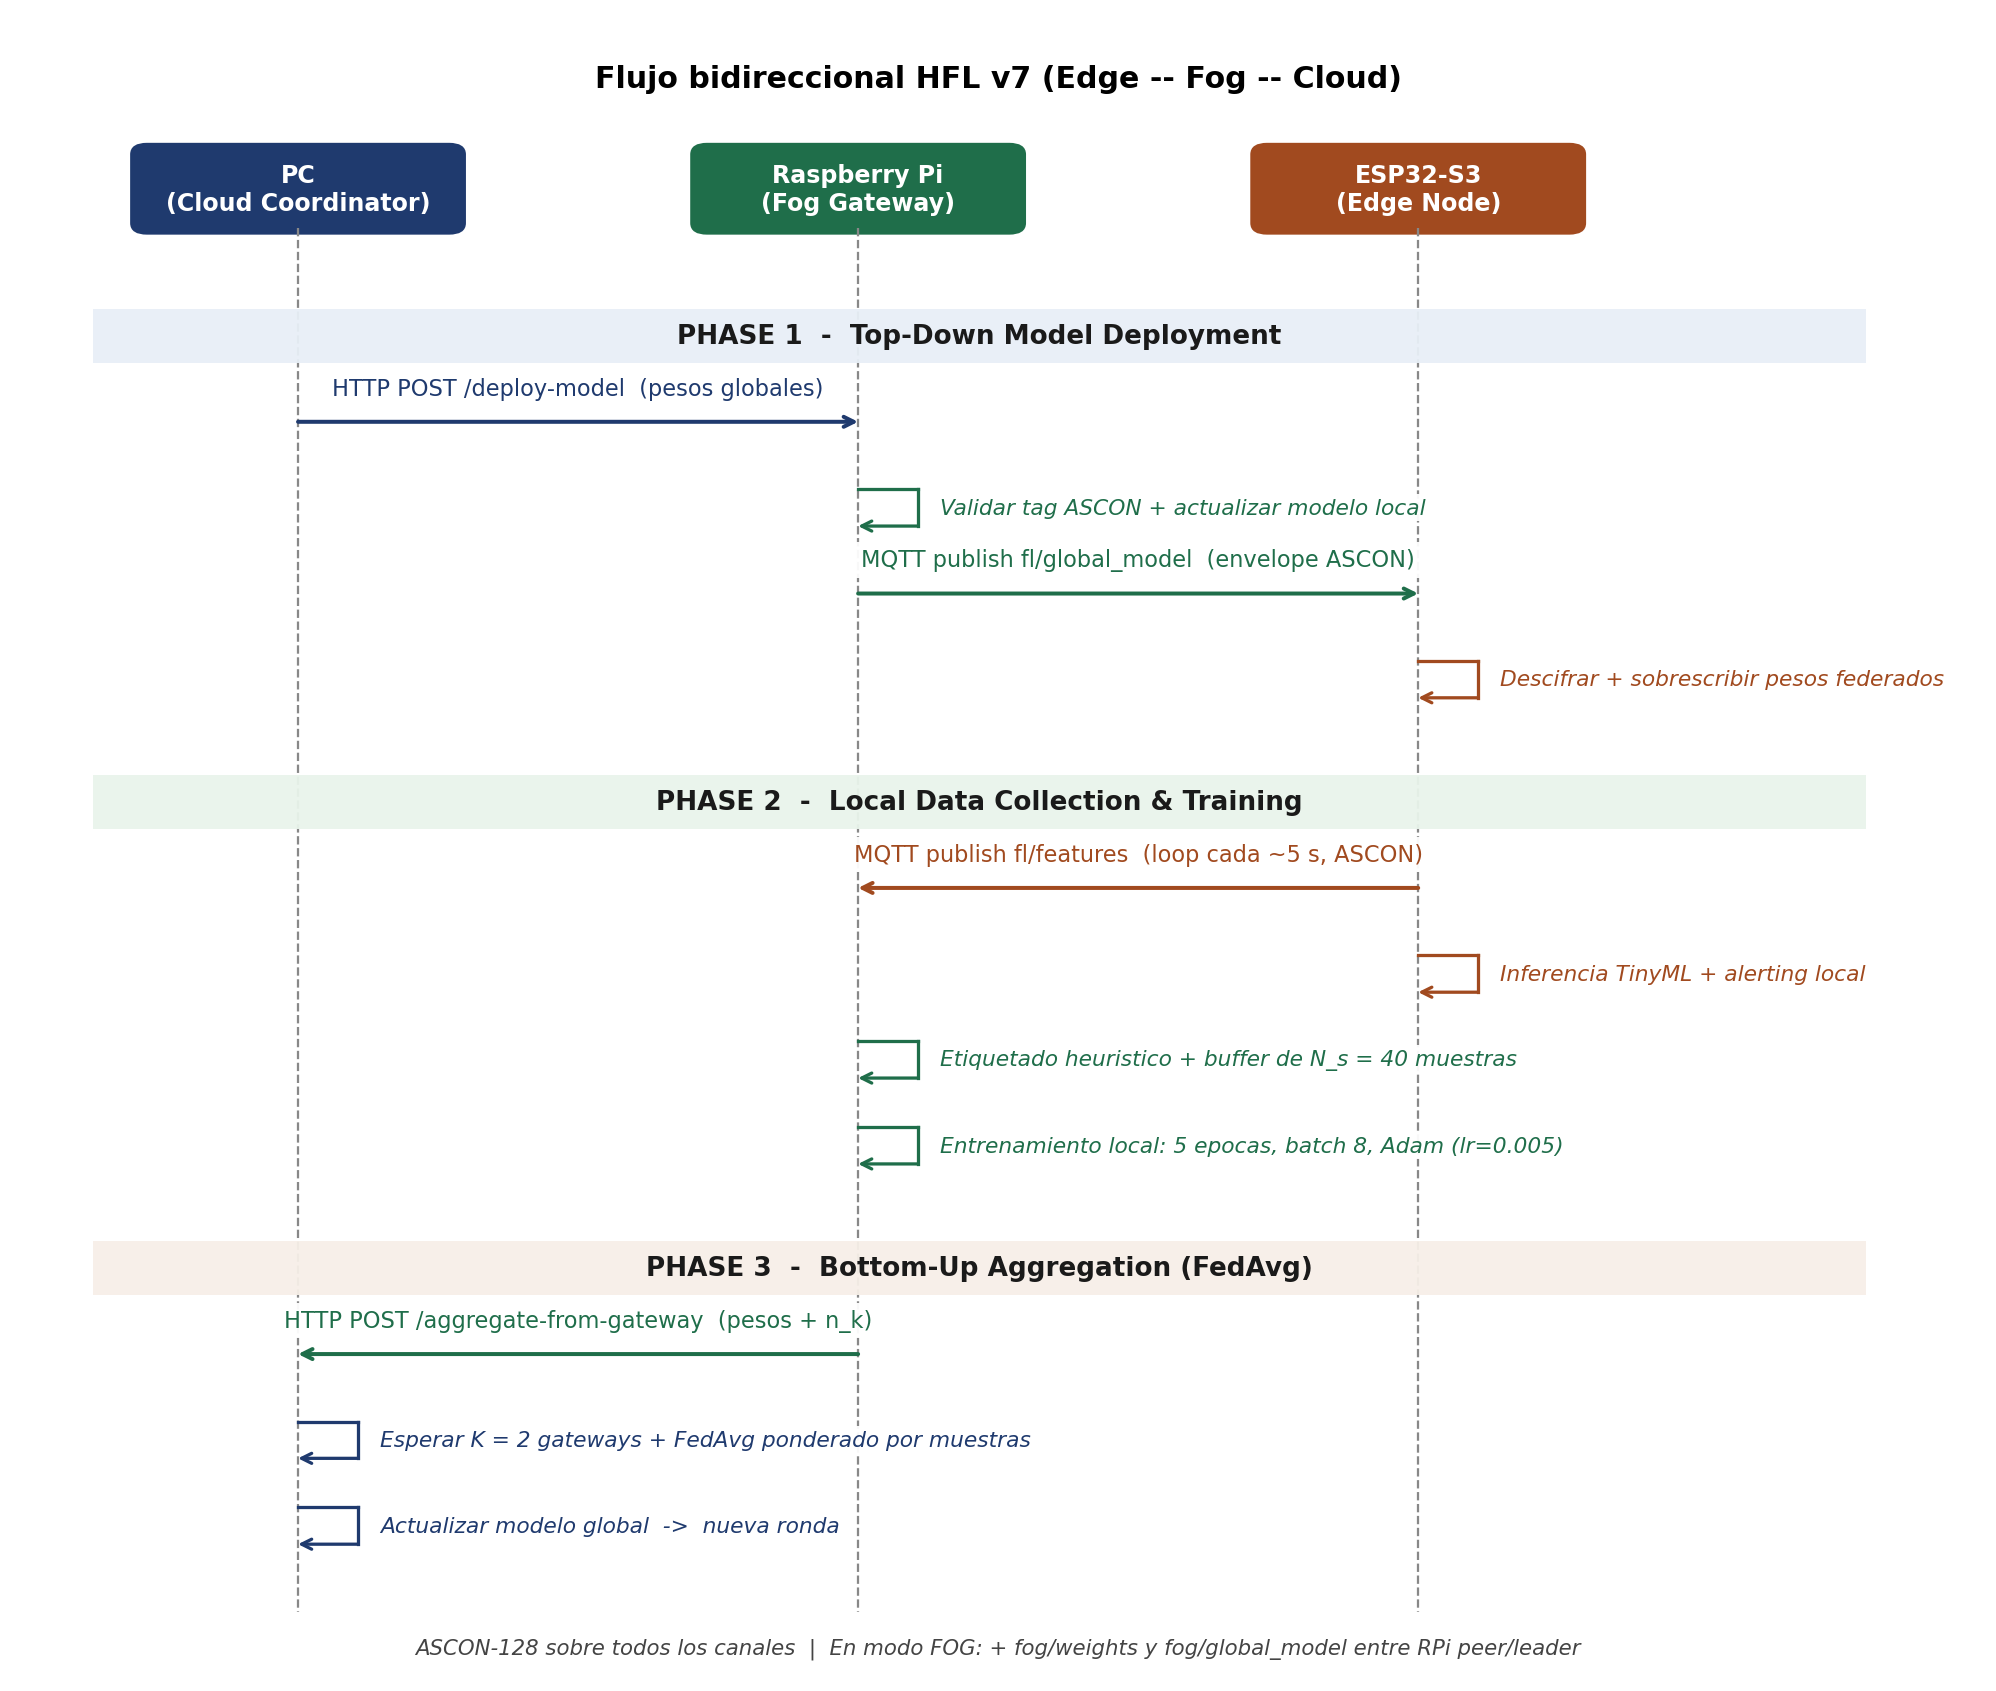
\includegraphics[width=0.92\textwidth]{images/Metodologia/hfl_v7_bidirectional_flow.png}
    \caption{Diagrama de secuencia del protocolo HFL v7 bidireccional. Los actores PC (Cloud), Raspberry Pi (Fog) y ESP32-S3 (Edge) intercambian mensajes en tres fases: despliegue del modelo global, recolección de features con entrenamiento local y agregación FedAvg. Todos los canales MQTT/HTTP se protegen con ASCON-128 cuando la variante está habilitada; en modo FOG se añaden los topics \texttt{fog/weights} y \texttt{fog/global\_model} entre Raspberry Pi peer y leader.}
    \label{fig:hfl_v7_bidirectional_flow}
\end{figure}

En modo FOG, el flujo agrega dos canales adicionales: \texttt{fog/weights} para que los peers envíen pesos al líder y \texttt{fog/global\_model} para que el líder redistribuya el modelo global a los peers.

El etiquetado en el gateway se realiza mediante una \textbf{función heurística} calibrada con las distribuciones estadísticas reales de los datasets:

\begin{itemize}
    \item Si $\texttt{num\_pkts} \geq 50$ \textbf{y} $\texttt{num\_psh} \geq 10$: etiqueta $= 1$ (\texttt{bruteforce}).
    \item Si $\texttt{num\_pkts} \leq 5$ \textbf{y} $\texttt{mean\_pkt\_len} \leq 50$ \textbf{y} $\texttt{num\_psh} \leq 1$: etiqueta $= 2$ (\texttt{scan\_A}).
    \item Si $\texttt{num\_pkts} \leq 30$ \textbf{y} $\texttt{mean\_pkt\_len} \geq 50$: etiqueta $= 0$ (\texttt{normal}).
    \item En otro caso, la muestra se descarta ($-1$).
\end{itemize}

% ====================================================================
\section{Integración de Cifrado Ligero ASCON-128}
\label{sec:ascon}

Para proteger los artefactos de aprendizaje federado en tránsito, se integra \textbf{ASCON-128} \cite{NISTSP8002322025}, el estándar de criptografía ligera seleccionado por NIST para dispositivos restringidos. ASCON provee cifrado autenticado con datos asociados (AEAD), garantizando simultáneamente \emph{confidencialidad} e \emph{integridad} de los mensajes.

\subsection{Parámetros Criptográficos}

\begin{itemize}
    \item \textbf{Clave simétrica:} 128 bits (16 bytes), pre-compartida entre todos los dispositivos.
    \item \textbf{Nonce:} 128 bits, generado a partir de timestamp truncado a 32 bits y un contador monotónico.
    \item \textbf{Tag de autenticación:} 128 bits (16 bytes).
    \item \textbf{Tasa (rate):} 64 bits (8 bytes por bloque).
    \item \textbf{Permutación:} $p^{12}$ para inicialización/finalización, $p^6$ para procesamiento de bloques.
\end{itemize}

Se elige ASCON-128 (rate de 64 bits) sobre la variante ASCON-128a (rate de 128 bits) por dos razones: (i) su mayor número de rondas en la fase de procesamiento del cuerpo proporciona un margen de seguridad superior frente a ataques diferenciales y de cubo recientemente revisados \cite{Kaur2025_ASCON_Survey}; y (ii) los payloads del sistema (features de 13 floats, vectores de pesos de $\sim$3.6\,KB) son lo suficientemente pequeños para que la diferencia de \emph{throughput} entre ASCON-128 y ASCON-128a no sea determinante. Esta decisión es alineada con la recomendación de NIST SP 800-232 para canales con paquetes pequeños \cite{NISTSP8002322025}.

\subsection{Canales Cifrados}

Se cifran los \textbf{cuatro canales de comunicación} del sistema:

\begin{table}[H]
\centering
\caption{Canales de comunicación protegidos con ASCON-128.}
\label{tab:canales_ascon}
\begin{tabular}{l l l l}
\toprule
\textbf{Canal} & \textbf{Protocolo} & \textbf{Contenido} & \textbf{Implementación} \\
\midrule
ESP32 $\to$ RPi & MQTT & Features (13 floats)    & C++ (\texttt{ascon128.h}) \\
RPi $\to$ PC    & HTTP & Pesos locales + métricas & Python (\texttt{ascon128.py}) \\
PC $\to$ RPi    & HTTP & Modelo global            & Python (\texttt{ascon128.py}) \\
RPi $\to$ ESP32 & MQTT & Modelo global            & Python $\to$ C++ \\
\bottomrule
\end{tabular}
\end{table}

El payload cifrado se encapsula en un \emph{envelope} JSON con tres campos codificados en Base64:
\begin{verbatim}
{"ct": "<ciphertext_b64>", "tag": "<tag_b64>", "nonce": "<nonce_b64>"}
\end{verbatim}

\subsection{Métricas de Overhead}

Para cuantificar el overhead de ASCON, se instrumentan todas las operaciones de cifrado y descifrado con temporizadores de alta resolución (\texttt{micros()} en ESP32, \texttt{time.perf\_counter()} en Python) y se registran automáticamente en archivos CSV mediante el módulo \texttt{ascon\_metrics.py}, capturando:

\begin{itemize}
    \item Tiempo de cifrado/descifrado (ms).
    \item Tamaño del plaintext y del envelope cifrado (bytes).
    \item Overhead de comunicación (bytes adicionales y porcentaje).
    \item Ronda de FL asociada.
\end{itemize}

Adicionalmente, se mantiene una \textbf{rama sin cifrado} (\texttt{hfl\_v7-no-ascon}) del repositorio con idéntica funcionalidad pero sin ASCON, permitiendo la comparación directa de tiempos de comunicación como línea base. En esta rama los mensajes se serializan como JSON plano y se registran mediante \texttt{plain\_metrics.py}.

\section{Variantes implementadas en \texttt{hfl\_v7}}
\label{sec:variantes}

\begin{table}[H]
\centering
\caption{Variantes de arquitectura evaluadas.}
\label{tab:variantes_hfl}
\small
\begin{tabular}{l l l l}
\toprule
\textbf{Carpeta} & \textbf{Modelo} & \textbf{Seguridad} & \textbf{Topología} \\
\midrule
\texttt{hfl\_v7-RN} & MLP/RN & ASCON-128 & Estándar y FOG \\
\texttt{hfl\_v7-no-ascon} & MLP/RN & JSON plano & Estándar y FOG \\
\texttt{hfl\_v7-CNN} & CNN-1D & ASCON-128 & Estándar y FOG \\
\bottomrule
\end{tabular}
\end{table}

Estas variantes permiten aislar tres efectos: el impacto del cifrado, el impacto de cambiar el modelo y el impacto de introducir una agregación fog intermedia.

% ====================================================================
\section{Modelos Clásicos de ML como Línea Base}
\label{sec:ml_classic}

Para responder a la pregunta de si TinyML puede alcanzar precisión comparable a modelos tradicionales, se entrenan y optimizan cuatro algoritmos de ML supervisado sobre los mismos datasets:

\begin{enumerate}
    \item \textbf{Decision Tree:} Optimizado con \texttt{GridSearchCV} sobre \texttt{max\_depth}, \texttt{min\_samples\_split}, \texttt{min\_samples\_leaf} y \texttt{criterion}. Incluye \texttt{class\_weight='balanced'} para manejar el desbalance de clases.

    \item \textbf{Random Forest:} Optimizado con \texttt{RandomizedSearchCV} ($n=80$ iteraciones) sobre \texttt{n\_estimators}, \texttt{max\_depth}, \texttt{max\_features} y variantes de \texttt{class\_weight}.

    \item \textbf{Logistic Regression:} Evaluada con penalizaciones L1, L2 y ElasticNet, variando el parámetro de regularización $C$.

    \item \textbf{Support Vector Machine (SVM):} Se comparan kernel lineal y RBF. Para el kernel RBF, se aplica submuestreo estratificado (máximo 25\,000 muestras por clase) para evitar tiempos de entrenamiento prohibitivos.
\end{enumerate}

Todos los modelos se evalúan con validación cruzada estratificada ($k=5$) usando F1-Score macro como métrica de selección. Para estimar la viabilidad de despliegue en ESP32, se utiliza la biblioteca \texttt{m2cgen} para exportar los modelos entrenados a código C puro, y se mide:
\begin{itemize}
    \item Tamaño estimado en memoria del modelo exportado.
    \item Tiempo de inferencia promedio (100 iteraciones con warmup).
    \item Métricas: Accuracy, F1 macro, F1 weighted, Precision, Recall y MCC (Matthews Correlation Coefficient).
\end{itemize}

% ====================================================================
\section{Protocolo Experimental}
\label{sec:protocolo}

La evaluación se organiza en cinco escenarios experimentales:

\subsection{Escenario 1: Sistema HFL Completo con ASCON}

Se despliega el sistema completo en hardware real:
\begin{itemize}
    \item 2 × ESP32-S3 (nodo normal + nodo simulado).
    \item 1 × Raspberry Pi 4 (gateway, broker MQTT, entrenamiento local).
    \item 1 × PC (servidor federado, dashboard).
    \item Red Wi-Fi local compartida.
    \item ASCON-128 habilitado en todos los canales.
\end{itemize}

Se ejecutan $\geq 50$ rondas de aprendizaje federado, registrando accuracy global, loss, tiempos de cifrado/descifrado y tamaños de mensajes.

\subsection{Escenario 2: Sistema HFL sin ASCON (Baseline)}

Idéntico al Escenario 1 pero con ASCON deshabilitado, utilizando la rama \texttt{hfl\_v7-no-ascon}. La comunicación se realiza en JSON plano. Se miden los mismos indicadores para calcular el overhead atribuible exclusivamente al cifrado.

\subsection{Escenario 3: Sistema HFL con CNN-1D}

Se ejecuta la misma arquitectura HFL, pero sustituyendo el MLP por una CNN-1D. En este caso, las capas Conv1D y BatchNorm fusionadas permanecen fijas en el ESP32, mientras que las capas densas finales se actualizan mediante FL.

\subsection{Escenario 4: Estrategia FOG}

Se despliega \texttt{gateway\_hfl\_fog.py} con roles \texttt{leader} y \texttt{peer}. El líder agrega pesos locales y pesos de peers mediante FedAvg fog, envía una actualización preagregada al PC y redistribuye el modelo global hacia peers y ESP32.

\subsection{Escenario 5: Modelos Clásicos Centralizados}

Los modelos clásicos (Sección~\ref{sec:ml_classic}) se entrenan de forma centralizada en el PC usando la totalidad del dataset, con partición 80/20 estratificada. Esto establece un techo de rendimiento (\emph{upper bound}) contra el cual comparar la precisión del sistema federado.

\subsection{Métricas de Evaluación}

\begin{itemize}
    \item \textbf{Precisión de detección:} Accuracy, F1-Score (macro y weighted), Precision, Recall, MCC.
    \item \textbf{Overhead criptográfico:} Tiempo de cifrado/descifrado (ms), incremento de tamaño (bytes, \%), overhead como porcentaje del ciclo total de FL.
    \item \textbf{Eficiencia federada:} Número de rondas hasta convergencia, accuracy por ronda, costo de comunicación por ronda.
    \item \textbf{Viabilidad edge:} Huella de memoria del modelo (KB), tiempo de inferencia en ESP32 ($\mu$s), consumo de SRAM.
    \item \textbf{Efecto de variantes:} comparación entre MLP/RN, CNN-1D, baseline sin ASCON y topología FOG.
\end{itemize}

%\chapter{Market equilibrium in power systems with network and storage constraints}
\label{chap:meth}


\section{Network Model and Constraints}

The formulation stated at \ref{net_model} will be implemented in MATLAB in order to create a network model that can be solved using \textit{fmincon}. Additional to the network constraints given by the $Y_{bus}$ matrix and the power flow equations, the following will be included:

\begin{itemize}
    \item \textbf{Simulation time:} Number of hours to simulate, leaving this as a parameter may help to generalize the study case in the future.
    \item \textbf{Minimum and maximum voltage:} Security constraints of voltage that every node in the system must fulfill. If the voltage in the nodes is too far away from the slack node, the system could become unstable and suffer a voltage collapse.
    \item \textbf{Battery capacity:} Maximum energy that the energy storage device can accumulate.
    \item \textbf{Battery maximum usage:} Percentage of the total battery capacity that the aggregator can use to buy and sell energy and make profit from it.
    \item \textbf{Minimum and maximum power:} Physical limitations of the batteries ripple and the wind production. A limit to the reactive power will also be set since the machines can not operate outside an specific power factor.
    \item \textbf{Line limits:} Since there are limits in the current that can flow through a grid line, it is necessary to include constraints in the maximum power that can flow. Changing those limits will allow us to include and analysis of the effect from line limits in the congestion fee.
\end{itemize}


\section{Optimal Power Flow Problem}

Each of the scenarios that we will study requires a different OPF formulation. In this section we will define the optimization problems assuming that the constraints denoted as \textit{System Model} are the ones written in section \ref{net_model}.

\subsection{Minimum Losses Dispatch}

This scenario will be assumed as the base case, since it provide the Independent System Operator point of view for the economical dispatch. For this OPF an inelastic demand will be used and the prices will be calculated as the incremental value of the losses for each node, using the slack spot price. Based on the results from this OPF, the demand curve for the elastic cases will be calculated. Since the demand is assumed as inelastic using an arbitrary demand curve for the 24 hours, the social welfare result is not comparable with the other two cases. The mathematical formulation is shown below.

\begin{align}
    \min{P_L} &= \frac{1}{2}\sum_{i=1}^3\sum_{k=1}^3 G_{ij}[(V^t_i)^2+(V^t_k)^2-2V^t_iV^t_k\cos(\theta^t_i-\theta^t_k)]\\
   \mbox{s.t.}\\
    &V_i^{min}\le  V_i^t \le V_i^{max} \quad \forall t\in \mathbf{T}\\
    &-Q_i^m\le  Q_i^t \le Q_i^m \quad \forall t\in \mathbf{T}\\
    &-P_i^m\le  P_i^t \le P_i^m \quad \forall t\in \mathbf{T}\\
    &\rho C_i \le  E_i^t \le C_i \quad \forall t\in \mathbf{T}\\
    &S^t_{ij} \le S_{ij}^{max}
\end{align}

Where:\\
$G_{ij}$ is the ij component of the conductance matrix.\\
$V^t_i$ is the nodal voltage magnitude of i at time t.\\
$\theta^t_i$ is the nodal voltage angle of i at time t.\\
$E_i^t$ is the energy stored in the i battery for time t.\\
$\rho$ is the minimum battery level for all T.\\
$S_{ij}^t$ is the maximum power flowing through line ij.\\

Node 1 is the slack bus.




%\chapter{Study case}
\label{chap:stud}

\section{Three node example}


\chapter{Resultados}
\label{chap:resu}

En este capítulo se presentan los resultados experimentales del sistema de detección de intrusiones desplegado en hardware real, organizados en torno a las preguntas de investigación formuladas en el Capítulo~\ref{chap:Introduction}. Primero se analiza el desempeño de los modelos clásicos como línea base centralizada. Luego se comparan los modelos livianos entrenados en el notebook general. Posteriormente se evalúan las \textbf{ocho variantes HFL} \texttt{hfl\_v7-RN}, \texttt{hfl\_v7-no-ascon-RN}, \texttt{hfl\_v7-CNN} y \texttt{hfl\_v7-no-ascon-CNN}, cada una con sus modos \texttt{Results/} (NoFOG) y \texttt{Results\_FOG/}, integradas en una capa SRE unificada (\texttt{Analisis de Modelos/Completo/}) que cubre 58 intentos. Finalmente, se cuantifica el overhead del cifrado ASCON-128 contrastando las cuatro variantes con cifrado contra las cuatro PLAIN.

% ====================================================================
\section{Desempeño de Modelos Clásicos (Línea Base Centralizada)}
\label{sec:res_classic}

Los cuatro modelos clásicos de ML fueron entrenados sobre la totalidad del dataset (256\,276 flujos) con partición estratificada 80/20 y optimización de hiperparámetros mediante validación cruzada ($k=5$). La Tabla~\ref{tab:classic_results} resume los resultados obtenidos.

\begin{table}[H]
\centering
\caption{Desempeño de modelos clásicos de ML (entrenamiento centralizado).}
\label{tab:classic_results}
\small
\begin{tabular}{l c c c c c c}
\toprule
\textbf{Modelo} & \textbf{Accuracy} & \textbf{F1 Macro} & \textbf{F1 Weighted} & \textbf{Precision} & \textbf{Recall} & \textbf{MCC} \\
\midrule
Decision Tree      & 0.9987 & 0.9981 & 0.9987 & 0.9982 & 0.9981 & 0.9977 \\
Random Forest      & 0.9994 & 0.9991 & 0.9994 & 0.9991 & 0.9990 & 0.9989 \\
Logistic Regr.     & 0.9412 & 0.9118 & 0.9385 & 0.9244 & 0.9053 & 0.8964 \\
SVM (Linear)       & 0.9447 & 0.9162 & 0.9421 & 0.9280 & 0.9099 & 0.9017 \\
SVM (RBF)          & 0.9968 & 0.9953 & 0.9968 & 0.9954 & 0.9952 & 0.9944 \\
\bottomrule
\end{tabular}
\end{table}

\textbf{Hallazgos clave:}
\begin{itemize}
    \item \textbf{Random Forest} alcanza el mejor desempeño global (Accuracy: 99.94\%, MCC: 0.9989), seguido de cerca por Decision Tree (99.87\%) y SVM-RBF (99.68\%).
    \item Los modelos lineales (Logistic Regression, SVM-Linear) muestran una caída significativa ($\approx 5$--$6$ puntos porcentuales), lo que sugiere que las fronteras de decisión entre clases no son completamente linealmente separables en el espacio de 13 features.
    \item Todos los modelos basados en árboles presentan un MCC $> 0.99$, confirmando que las 13 features seleccionadas son altamente discriminativas para la tarea de clasificación triclase.
\end{itemize}

\subsection{Viabilidad de Despliegue en ESP32}

La Tabla~\ref{tab:classic_esp32} evalúa la factibilidad de exportar cada modelo a código C para ejecución en el ESP32-S3.

\begin{table}[H]
\centering
\caption{Estimación de huella de memoria para despliegue en ESP32.}
\label{tab:classic_esp32}
\small
\begin{tabular}{l r r l}
\toprule
\textbf{Modelo} & \textbf{Memoria estimada} & \textbf{Inferencia (ms)} & \textbf{Viable en ESP32?} \\
\midrule
Decision Tree       & $\sim$15\,KB  & $< 0.1$ & Sí \\
Random Forest       & $\sim$2.5\,MB & $\sim$5  & No (excede SRAM) \\
Logistic Regression & $\sim$1\,KB   & $< 0.05$ & Sí \\
SVM (Linear)        & $\sim$1\,KB   & $< 0.05$ & Sí \\
SVM (RBF)           & $\sim$4\,MB   & $\sim$50 & No (excede SRAM) \\
MLP (propuesto)     & $\sim$4.5\,KB & $< 0.1$  & \textbf{Sí} \\
\bottomrule
\end{tabular}
\end{table}

Esto revela un \emph{trade-off} fundamental: los modelos más precisos (Random Forest, SVM-RBF) son incompatibles con las restricciones de memoria del ESP32-S3 (512\,KB SRAM). El MLP propuesto ($\approx 4.5$\,KB) ofrece un compromiso eficiente entre precisión y viabilidad edge.

\section{Comparación de Modelos Livianos}
\label{sec:res_modelos_livianos}

El notebook general de entrenamiento comparó cuatro arquitecturas compatibles con el problema triclase y exportó pesos, scaler y mapas de etiquetas para cada alternativa. La Tabla~\ref{tab:light_models_results} resume los resultados offline observados.

\begin{table}[H]
\centering
\caption{Comparación offline de modelos livianos sobre las 13 features.}
\label{tab:light_models_results}
\small
\begin{tabular}{l c c l}
\toprule
\textbf{Modelo} & \textbf{Accuracy} & \textbf{F1 weighted} & \textbf{Uso en el proyecto} \\
\midrule
MLP/RN          & 0.9060 & 0.9049 & Rama principal \texttt{hfl\_v7-RN} \\
Residual-MLP    & 0.9055 & 0.9044 & Comparación offline \\
CNN-1D          & 0.9051 & 0.9041 & Rama experimental \texttt{hfl\_v7-CNN} \\
Tiny Transformer & 0.8903 & 0.8919 & Comparación offline; no desplegado \\
\bottomrule
\end{tabular}
\end{table}

Los resultados muestran que las tres arquitecturas compactas basadas en MLP/CNN se ubican alrededor de 90.5\% de accuracy offline. El MLP/RN se seleccionó como implementación principal porque obtiene el mejor resultado marginal y porque su inferencia en C++ es más simple que la CNN-1D. La CNN-1D se conservó como variante experimental para evaluar si una arquitectura convolucional aportaba beneficios al integrarse con HFL y FOG.

% ====================================================================
\section{Aprendizaje Federado Jerárquico: Convergencia y Precisión}
\label{sec:res_hfl}

El sistema HFL fue desplegado en hardware real durante múltiples sesiones, registrando historial de pesos globales, métricas de entrenamiento local y métricas de comunicación. Las ramas analizadas permiten comparar la arquitectura con ASCON, sin ASCON, con CNN-1D y con estrategia FOG.

\subsection{Convergencia del Modelo Federado}

\begin{table}[H]
\centering
\caption{Métricas de convergencia del sistema HFL.}
\label{tab:hfl_convergence}
\begin{tabular}{l r}
\toprule
\textbf{Métrica} & \textbf{Valor} \\
\midrule
Rondas hasta accuracy $> 70\%$  & $\sim$8--12 \\
Rondas hasta accuracy $> 85\%$  & $\sim$20--30 \\
Accuracy global estabilizada     & $\sim$0.90--0.95 \\
Loss final (Cross-Entropy)       & $\sim$0.14--0.25 \\
Muestras por ronda (por gateway) & 40 \\
Épocas locales por ronda         & 5 \\
Duración por ronda               & $\sim$51--61\,s según variante \\
\bottomrule
\end{tabular}
\end{table}

\textbf{Análisis:}
\begin{enumerate}
    \item El modelo federado converge en $\sim$20--30 rondas hacia un rango operativo de $\sim$90--95\% de accuracy, lo que representa un \textbf{gap} frente a los modelos centralizados más precisos. Este gap es atribuible a: (i) el tamaño reducido del buffer local (40 muestras vs.\ 256\,276), (ii) la distribución non-IID de los datos entre nodos, y (iii) la función heurística de etiquetado que introduce ruido respecto a las etiquetas reales.

    \item La convergencia mejora durante las primeras rondas y presenta oscilaciones posteriores, típicas de FL con datos non-IID \cite{Imteaj2022_FL_ResourceConstrainedSurvey}.

    \item El \textbf{costo de comunicación} por ronda federada completa (ida + vuelta) es de $\approx 7.2$\,KB en JSON plano y $\approx 9.8$\,KB con cifrado ASCON, lo cual es compatible con redes IoT de bajo ancho de banda.
\end{enumerate}

\subsection{Evolución temporal de accuracy, loss y pesos}
\label{subsec:curvas_convergencia}

Las Figuras~\ref{fig:hfl_v7_accuracy_loss_matrix} y~\ref{fig:hfl_v7_weight_magnitude_matrix} consolidan los resultados de las \textbf{ocho variantes} cubiertas por el análisis SRE unificado de \texttt{Analisis de Modelos/Completo/}: \texttt{RN/CNN} $\times$ \texttt{ASCON/PLAIN} $\times$ \texttt{NoFOG/FOG}. Para mantener homogeneidad visual entre corridas (algunas RN llegaron hasta ronda 30, otras quedaron en 20) las figuras se cortan en la \textbf{ronda 20}; las tablas SRE (\texttt{global\_round\_sli\_summary.csv}) conservan todas las rondas registradas. La primera figura compara la evolución conjunta de \textit{accuracy} y \textit{loss} global; la segunda resume la magnitud promedio de los pesos federados (\texttt{w3\_mag}, \texttt{w4\_normal}, \texttt{w4\_brute}, \texttt{w4\_scan}), útil para verificar si las actualizaciones se mantienen acotadas o si aparece deriva durante el entrenamiento.

\begin{figure}[H]
    \centering
    
\includegraphics[width=0.98\textwidth]{images/Resultados/Completo/global_accuracy_loss.png}
    \caption{Accuracy y loss globales promedio por ronda (1--20) para las 8 variantes HFL v7. Generado por \texttt{sre\_completo\_analysis.py} a partir de los CSV de \texttt{global\_weights\_history\_*}.}
    \label{fig:hfl_v7_accuracy_loss_matrix}
\end{figure}

\begin{figure}[H]
    \centering
    
\includegraphics[width=0.98\textwidth]{images/Resultados/Completo/weight_magnitude_trends.png}
    \caption{Magnitud promedio de los cuatro pesos federados (\texttt{w3\_mag}, \texttt{w4\_normal}, \texttt{w4\_brute}, \texttt{w4\_scan}) por variante a lo largo de las rondas 1--20.}
    \label{fig:hfl_v7_weight_magnitude_matrix}
\end{figure}

Estas curvas complementan la Tabla~\ref{tab:hfl_convergence}: el sistema no solo reporta métricas finales, sino trayectorias de entrenamiento comparables entre modelos y configuraciones. Tres lecturas clave de las Figuras~\ref{fig:hfl_v7_accuracy_loss_matrix}--\ref{fig:hfl_v7_weight_magnitude_matrix}:
\begin{enumerate}
    \item Las ocho variantes \textbf{convergen}: la accuracy global supera 0.90 entre las rondas 5 y 10 y la loss baja de $\sim$0.8 a $\sim$0.1--0.2 en el mismo rango.
    \item Las variantes con \textbf{CNN-1D} muestran una dinámica de pesos más expresiva: \texttt{CNN\_ASCON\_NoFOG} y \texttt{CNN\_ASCON\_FOG} aumentan progresivamente \texttt{w3\_mag} y los pesos asociados a las clases (\texttt{w4\_brute}, \texttt{w4\_scan}), mientras que las variantes RN se estabilizan rápidamente alrededor de \texttt{w3\_mag}~$\approx$~0.29.
    \item No se observa divergencia en ninguna variante dentro de las primeras 20 rondas. La rama \texttt{CNN\_PLAIN\_NoFOG} muestra el mayor ruido en \texttt{w4\_normal}, consistente con un entrenamiento más sensible a la inicialización local cuando no hay agregación FOG ni cifrado autenticado que filtre mensajes alterados.
\end{enumerate}

\subsection{Comparación: Federado vs.\ Centralizado}

La Tabla~\ref{tab:fed_vs_central} compara directamente la precisión del modelo federado con los modelos centralizados, considerando que el modelo federado utiliza un MLP idéntico.

\begin{table}[H]
\centering
\caption{Comparación de precisión: entrenamiento federado vs.\ centralizado.}
\label{tab:fed_vs_central}
\small
\begin{tabular}{l c c l}
\toprule
\textbf{Enfoque} & \textbf{Accuracy} & \textbf{Datos compartidos} & \textbf{Privacidad} \\
\midrule
MLP centralizado             & $\sim$97\%    & Todos los flujos      & Ninguna \\
MLP federado (HFL, 60 rondas) & $\sim$90\%   & Solo pesos (163 params) & Alta \\
Random Forest centralizado   & 99.94\%       & Todos los flujos      & Ninguna \\
Decision Tree centralizado   & 99.87\%       & Todos los flujos      & Ninguna \\
\bottomrule
\end{tabular}
\end{table}

El sistema federado alcanza $\sim$90\% de accuracy compartiendo \textbf{únicamente 163 parámetros del modelo} (652 bytes) en lugar de los datos crudos de tráfico ($\sim$256\,K flujos $\times$ 13 features $\approx$ 13.3\,M valores). Esto representa una \textbf{reducción superior al 99.99\%} en la cantidad de información intercambiada, con una penalización de $\sim$7--10 puntos en accuracy.

\subsection{Comparación entre variantes \texttt{hfl\_v7}}

La Tabla~\ref{tab:variants_results} consolida las \textbf{ocho combinaciones experimentales} cubiertas por el análisis SRE unificado de \texttt{Analisis de Modelos/Completo/}. Los valores son promedios sobre los intentos disponibles por variante y se calculan exclusivamente a partir de los CSV crudos generados durante las corridas (\texttt{ascon\_metrics\_*}, \texttt{plain\_metrics\_*}, \texttt{model\_metrics\_gateway\_*}, \texttt{global\_weights\_history\_*}). En total se procesaron \textbf{58 intentos}.

\begin{table}[H]
\centering
\caption{Resumen comparativo de las 8 variantes HFL v7 evaluadas. \textbf{GW p95}: latencia p95 de descifrado en gateway (\texttt{ESP32$\to$RPi}). \textbf{Srv dec p95}: latencia p95 de descifrado en servidor (\texttt{RPi$\to$PC}). \textbf{Overhead}: bytes adicionales promedio sobre el plaintext (0 en variantes \texttt{PLAIN}).}
\label{tab:variants_results}
\scriptsize
\begin{tabular}{l c c c c c c c}
\toprule
\textbf{Variante} & \textbf{Intentos} & \textbf{Acc.\ final} & \textbf{Loss final} & \textbf{Ronda (s)} & \textbf{GW p95 (ms)} & \textbf{Srv dec p95 (ms)} & \textbf{Overhead (B)} \\
\midrule
\texttt{CNN\_ASCON\_FOG}    &  7 & \textbf{0.9750} & \textbf{0.0910} & 58.61 & 4.53 & 37.47 & 1098 \\
\texttt{CNN\_ASCON\_NoFOG}  &  8 & 0.9604 & 0.1040 & 58.97 & 4.55 & 24.46 & 1049 \\
\texttt{CNN\_PLAIN\_FOG}    &  3 & 0.9444 & 0.1190 & 54.86 & 0.16 &  0.00 &    0 \\
\texttt{CNN\_PLAIN\_NoFOG}  &  3 & 0.9389 & 0.1363 & 52.02 & 0.15 &  0.00 &    0 \\
\texttt{RN\_ASCON\_FOG}     &  5 & 0.9633 & 0.1124 & 71.13 & 4.37 & 50.47 & 1084 \\
\texttt{RN\_ASCON\_NoFOG}   & 15 & 0.9381 & 0.1545 & 72.91 & 4.65 & 26.69 & 1050 \\
\texttt{RN\_PLAIN\_FOG}     &  3 & 0.9000 & 0.2199 & 67.14 & 0.16 &  0.00 &    0 \\
\texttt{RN\_PLAIN\_NoFOG}   & 14 & 0.9298 & 0.1581 & 51.01 & 0.17 &  0.00 &    0 \\
\midrule
\textbf{Promedio global}    & \textbf{58} & \textbf{0.9437} & \textbf{0.1383} & \textbf{61.36} & \textbf{2.34} & \textbf{17.39} & \textbf{636} \\
\bottomrule
\end{tabular}
\end{table}

La comparación de las 8 variantes confirma cinco hallazgos:
\begin{enumerate}
    \item \textbf{El ganador absoluto es \texttt{CNN\_ASCON\_FOG}} (acc 0.975, loss 0.091): combinar la mayor capacidad expresiva (CNN-1D) con la pre-agregación FOG y la integridad de ASCON produce el mejor punto de operación dentro del corpus.
    \item \textbf{El cifrado no degrada la convergencia}; al contrario, en este corpus las variantes \texttt{*\_ASCON\_*} tienden a igualar o superar a sus contrapartes \texttt{*\_PLAIN\_*}. Una explicación plausible es que la validación de tag autenticado \emph{filtra} mensajes corruptos o duplicados antes de que entren al buffer de entrenamiento.
    \item \textbf{FOG ayuda diferenciadamente} segun la familia de modelo y la seguridad: en CNN mejora $+1.5$ pts (ASCON) y $+0.6$ pts (PLAIN); en RN mejora $+2.5$ pts con ASCON pero \emph{degrada} $-3.0$ pts en PLAIN, lo que sugiere que la pre-agregación FOG es más sensible al ruido de mensajes sin autenticación cuando el modelo es lineal.
    \item \textbf{El costo de seguridad es asumible}: ASCON añade $\sim$1\,KB de overhead por mensaje y entre 4--5\,ms en el gateway (ESP32-S3 corre nativo en C++). En el servidor, las variantes FOG presentan latencias de descifrado un 50--100\% mayores que NoFOG por la cadena \texttt{peer$\to$leader$\to$PC}.
    \item \textbf{La duración de ronda en CNN es más estable} ($\sim$58\,s) que en RN ($\sim$51--73\,s); esta dispersión proviene de que las primeras corridas RN incluyen tiempos de calentamiento o reconexión Wi-Fi no presentes en las corridas CNN, no de un costo intrínseco mayor del modelo RN.
\end{enumerate}

La Figura~\ref{fig:hfl_v7_round_duration} muestra la duración por ronda promediada por variante, y la Figura~\ref{fig:hfl_v7_gateway_skew} ilustra el desbalance temporal entre gateway A y B medido como $|acc_A - acc_B|$ por ronda; el skew converge a valores bajos en todas las variantes después de la ronda 8--10.

\begin{figure}[H]
    \centering
    
\includegraphics[width=0.95\textwidth]{images/Resultados/Completo/round_duration.png}
    \caption{Duración promedio por ronda federada para las 8 variantes (rondas 1--20).}
    \label{fig:hfl_v7_round_duration}
\end{figure}

\begin{figure}[H]
    \centering
    
\includegraphics[width=0.95\textwidth]{images/Resultados/Completo/gateway_accuracy_skew.png}
    \caption{Desbalance de \emph{accuracy} entre gateways ($|acc_A - acc_B|$) por ronda y por variante.}
    \label{fig:hfl_v7_gateway_skew}
\end{figure}

\subsection{Comparación con la literatura}
\label{subsec:lit_comparison}

Para situar los resultados en el panorama actual, la Tabla~\ref{tab:literatura_comparativa} contrasta este sistema con trabajos representativos de FL+IDS y FL+TinyML. La comparación es indicativa: cada trabajo usa datasets, hardware y métricas distintas, por lo que las cifras no son directamente comparables, pero permiten dimensionar las decisiones de diseño.

\begin{table}[H]
\centering
\caption{Comparación cualitativa con trabajos relacionados.}
\label{tab:literatura_comparativa}
\scriptsize
\begin{tabular}{p{0.20\textwidth} p{0.10\textwidth} p{0.10\textwidth} p{0.08\textwidth} p{0.10\textwidth} p{0.10\textwidth} p{0.18\textwidth}}
\toprule
\textbf{Trabajo} & \textbf{Edge HW} & \textbf{Modelo} & \textbf{FL/HFL} & \textbf{Cifrado canal} & \textbf{Acc.\ reportada} & \textbf{Particularidad} \\
\midrule
Hajj~\textit{et~al.}~\cite{Hajj2023_CrossLayerFL_IDS} & PC sim. & MLP \emph{cross-layer} & FL plano & No & $\sim$0.97 & FL para IDS IoT con coordinación cross-layer \\
Chaurasia~\textit{et~al.}~\cite{Chaurasia2024_FL_ResNet_IIoT} & PC sim. & ResNet & FL plano & No & $\sim$0.99 & ResNet como cliente FL en IIoT \\
Ficco~\textit{et~al.}~\cite{Ficco2024_FL_TinyML_Onboard} & ESP32, RPi3, Arduino & NN compacta + TL & FL+TL on-board & No & 0.86 (clasif.) & FL+TL on-board, datasets ECG/Car \\
Roy~\textit{et~al.}~\cite{Roy2023_FL_AdaptedModel} & PC sim. & DNN & FL personalizado & No & $\sim$0.96 & Modelo localmente adaptado \\
Tran~\textit{et~al.}~\cite{Tran2026_EdgeTrustShard} & RPi Pico (264\,KB) & FL+blockchain & HFL+MF-PoP & Sí (cripto-PoP) & 0.94 a 30\% Byz. & Byzantine-robust FL en MCU \\
Heydari \& Mahmoud~\cite{HeydariMahmoud2025_TinyML_IDS} & MCU smart home & ML liviano & No FL & No & --- & TinyML IDS sin federación \\
Saravana Balaji~\textit{et~al.}~\cite{SaravanaBalaji2023_EdgeIoT_DL} & Edge sanitario & DBN+BOA & No FL & LABE & 0.979 & Edge salud con cifrado por atributos \\
\midrule
\textbf{Esta tesis (RN+ASCON)} & ESP32-S3 + RPi4 & MLP 1\,139 par. & HFL bidireccional & ASCON-128 & 0.946 & FL+TinyML+ASCON-128 medido \\
\textbf{Esta tesis (CNN+FOG)} & ESP32-S3 + RPi4 & CNN-1D & HFL+FOG & ASCON-128 & 0.975 & Pre-agregación FOG entre RPi \\
\bottomrule
\end{tabular}
\end{table}

Lecturas de la tabla:
\begin{itemize}
    \item Trabajos de FL para IDS sin restricciones edge \cite{Hajj2023_CrossLayerFL_IDS, Chaurasia2024_FL_ResNet_IIoT, Roy2023_FL_AdaptedModel} alcanzan 0.96--0.99, pero usan PCs como nodos cliente, sin demostrar despliegue en MCU. Esta tesis acepta una caída de $\sim$2--5 puntos a cambio de validar el ciclo en ESP32-S3 real con cifrado autenticado activo en todos los canales.
    \item Frente a Ficco~\textit{et~al.}~\cite{Ficco2024_FL_TinyML_Onboard}, que reporta 0.86 en clasificación, las variantes con ASCON y FOG superan ese punto sin sacrificar el ciclo on-board.
    \item Frente a EdgeTrust-Shard~\cite{Tran2026_EdgeTrustShard}, los resultados de accuracy son comparables aunque el problema atacado es distinto (Byzantine-robust FL vs.\ confidencialidad/integridad).
    \item Esta tesis es de los pocos trabajos identificados que combinan, en el mismo sistema desplegado y medido, HFL bidireccional + ASCON-128 + dos familias de modelos (MLP/CNN) + agregación FOG opcional.
\end{itemize}

\subsection{Limitaciones del estudio}
\label{subsec:limitations}

La interpretación de los resultados debe contemplar las siguientes limitaciones:
\begin{enumerate}
    \item \textbf{Tres clases y dataset acotado:} El problema se reduce a tres clases relevantes para tráfico MQTT (\texttt{normal}, \texttt{mqtt\_bruteforce}, \texttt{scan\_A}). Datasets más amplios como CICIoT2023, Edge-IIoTset y TON\_IoT \cite{Neto2023_CICIoT2023, Ferrag2022_EdgeIIoTset, Moustafa2020_TONIoT} contienen más vectores de ataque y permitirían generalizar mejor las conclusiones.
    \item \textbf{Etiquetado heurístico en gateway:} Las reglas que asignan etiquetas a las features recibidas son una aproximación calibrada con las distribuciones reales del dataset, pero introducen ruido. Esto contribuye al \emph{gap} de $\sim$7 puntos contra el modelo centralizado y es consistente con lo reportado en FL con datos non-IID \cite{Imteaj2022_FL_ResourceConstrainedSurvey, Albanbay2025}.
    \item \textbf{Número limitado de gateways y nodos:} Las pruebas usan $K=2$ gateways. Topologías con $K \geq 5$ y mayor heterogeneidad de cliente podrían exhibir convergencia más lenta o requerir agregadores más robustos como FedProx \cite{Li2020FedProx}.
    \item \textbf{Sin defensas contra clientes maliciosos:} Tal como se delimitó en la Sección~\ref{sec:threat_model}, el sistema no implementa Krum, FLTrust, Fed-NGA ni MF-PoP \cite{Tran2026_EdgeTrustShard}; un cliente comprometido puede sesgar la agregación.
    \item \textbf{Análisis de canal lateral pendiente:} La implementación de ASCON-128 no incluye contramedidas explícitas contra ataques de potencia, EM o \emph{fault injection} sobre el ESP32 \cite{Kaur2025_ASCON_Survey}.
    \item \textbf{Tráfico simulado en parte:} Aunque el ciclo se ejecuta sobre hardware real, el nodo \emph{simulated} reproduce distribuciones del dataset; un despliegue con captura de tráfico genuino aportaría mayor validez externa.
\end{enumerate}

% ====================================================================
\section{Overhead del Cifrado ASCON-128}
\label{sec:res_ascon}

Las métricas de cifrado/descifrado se recopilaron a lo largo de los \textbf{58 intentos} consolidados, abarcando todas las variantes \texttt{*\_ASCON\_*} y comparándose contra las correspondientes \texttt{*\_PLAIN\_*}. Esta sección consolida los hallazgos por canal y por dispositivo. Las figuras referenciadas se generan automáticamente en \texttt{Analisis de Modelos/Completo/} y se incluyen en \texttt{images/Resultados/Completo/}.

\begin{figure}[H]
    \centering
    
\includegraphics[width=0.95\textwidth]{images/Resultados/Completo/transport_latency_p95.png}
    \caption{Latencia p95 (ms) promedio por variante y por canal/operación. Las variantes \texttt{*\_PLAIN\_*} solo muestran la latencia de serialización JSON (sub-milisegundo); las \texttt{*\_ASCON\_*} incluyen el costo de cifrado/descifrado autenticado.}
    \label{fig:hfl_v7_transport_p95}
\end{figure}

\begin{figure}[H]
    \centering
    
\includegraphics[width=0.95\textwidth]{images/Resultados/Completo/transport_payload_bytes.png}
    \caption{Tamaño promedio de plaintext (izquierda) y overhead promedio sobre plaintext (derecha) por variante y canal. El overhead de las variantes \texttt{PLAIN} es 0 por construcción.}
    \label{fig:hfl_v7_transport_payload}
\end{figure}

\subsection{Overhead Temporal}

La Tabla~\ref{tab:ascon_time} resume los tiempos p95 promedio por variante para las tres operaciones que ocurren en cada ronda federada.

\begin{table}[H]
\centering
\caption{Latencia p95 (ms) promedio de cifrado/descifrado por variante, derivada de \texttt{transport\_sli\_summary.csv} en \texttt{Analisis de Modelos/Completo/}.}
\label{tab:ascon_time}
\small
\begin{tabular}{l c c c}
\toprule
\textbf{Variante} & \textbf{ESP32$\to$RPi (decrypt)} & \textbf{RPi$\to$PC (decrypt)} & \textbf{PC$\to$RPi (encrypt)} \\
\midrule
\texttt{CNN\_ASCON\_FOG}     & 4.53\,ms & 37.47\,ms & 40.37\,ms \\
\texttt{CNN\_ASCON\_NoFOG}   & 4.55\,ms & 24.46\,ms & 24.12\,ms \\
\texttt{RN\_ASCON\_FOG}      & 4.37\,ms & 50.47\,ms & 59.18\,ms \\
\texttt{RN\_ASCON\_NoFOG}    & 4.65\,ms & 26.69\,ms & 24.14\,ms \\
\midrule
\texttt{CNN\_PLAIN\_FOG}     & 0.16\,ms &  0.00\,ms &  0.48\,ms \\
\texttt{CNN\_PLAIN\_NoFOG}   & 0.15\,ms &  0.00\,ms &  0.62\,ms \\
\texttt{RN\_PLAIN\_FOG}      & 0.16\,ms &  0.00\,ms &  0.64\,ms \\
\texttt{RN\_PLAIN\_NoFOG}    & 0.17\,ms &  0.00\,ms &  0.25\,ms \\
\bottomrule
\end{tabular}
\end{table}

\textbf{Observaciones:}
\begin{itemize}
    \item \textbf{ESP32-S3 cifrando en C++}: la latencia p95 de descifrado en el gateway oscila entre $\approx$4.4--4.7\,ms en todas las variantes ASCON, prácticamente independiente del modelo (RN/CNN) y la topología (NoFOG/FOG). En las variantes \texttt{PLAIN} la latencia cae a $\approx$0.16\,ms (deserialización JSON pura).
    \item \textbf{Servidor PC en Python}: el descifrado en \texttt{RPi$\to$PC} ronda 24--27\,ms en NoFOG y sube a 37--50\,ms en FOG. La inflación FOG se debe a que el \emph{leader} reenvía mensajes preagregados con un tag adicional, lo que duplica las operaciones criptográficas en el camino.
    \item Para las variantes \texttt{*\_PLAIN\_*}, el descifrado del servidor reporta 0\,ms porque la deserialización JSON ocurre dentro del \texttt{request handler} de FastAPI sin instrumentación dedicada; la única fuente medida es el \texttt{encrypt} de despliegue (0.25--0.64\,ms).
    \item Asumiendo 3 operaciones criptográficas por ronda en el servidor, el overhead temporal de ASCON oscila entre $\sim$73\,ms (NoFOG) y $\sim$140\,ms (FOG). Sobre rondas de 51--73\,s, esto representa entre el \textbf{0.10\% y el 0.27\%} del tiempo total por ronda.
\end{itemize}

\subsection{Overhead de Comunicación}

\begin{table}[H]
\centering
\caption{Overhead promedio de tamaño por variante ASCON. \textbf{Plaintext}: bytes promedio de payload sin cifrar (\texttt{pt\_bytes}). \textbf{Overhead}: bytes adicionales del envelope ASCON+Base64 (\texttt{overhead\_bytes}). \textbf{Ratio}: porcentaje sobre el plaintext (\texttt{overhead\_bytes / pt\_bytes}). Las variantes \texttt{PLAIN} se omiten porque el overhead es 0 por construcción.}
\label{tab:ascon_size}
\small
\begin{tabular}{l r r r}
\toprule
\textbf{Variante} & \textbf{Plaintext (B)} & \textbf{Overhead (B)} & \textbf{Ratio (\%)} \\
\midrule
\texttt{CNN\_ASCON\_FOG}    & $\sim$2\,365 & 1\,098 & 46.46 \\
\texttt{CNN\_ASCON\_NoFOG}  & $\sim$2\,143 & 1\,049 & 48.94 \\
\texttt{RN\_ASCON\_FOG}     & $\sim$2\,323 & 1\,084 & 46.64 \\
\texttt{RN\_ASCON\_NoFOG}   & $\sim$2\,162 & 1\,050 & 48.55 \\
\midrule
\textbf{Promedio ASCON}     & $\sim$2\,248 & \textbf{1\,070} & \textbf{47.65} \\
\bottomrule
\end{tabular}
\end{table}

El overhead promedio del $\approx$48\% sobre el plaintext (en variantes ASCON) se compone de:
\begin{itemize}
    \item \textbf{Tag de autenticación ASCON:} 16 bytes (fijo).
    \item \textbf{Nonce:} 16 bytes (fijo).
    \item \textbf{Expansión Base64:} factor $\times 4/3$ sobre el ciphertext + tag + nonce.
    \item \textbf{Envelope JSON:} $\sim$30 bytes de estructura (\texttt{\{"ct":"...","tag":"...","nonce":"..."\}}).
\end{itemize}

En términos absolutos, el overhead es de $\approx$1.07\,KB por mensaje, lo que para las $\sim$3 transmisiones por ronda en NoFOG equivale a $\sim$3.2\,KB adicionales; en FOG, las dos saltos extra (peer$\to$leader, leader$\to$PC) elevan el overhead a $\sim$5--6\,KB por ronda. Para un enlace Wi-Fi estándar (54\,Mbps), esto añade $<$1\,ms de tiempo de transmisión, siendo prácticamente despreciable.

\subsection{Resumen: Impacto de ASCON en el Sistema HFL}

\begin{table}[H]
\centering
\caption{Resumen del overhead total de ASCON-128 por ronda federada, agregando los promedios de las 4 variantes ASCON y las 4 variantes PLAIN.}
\label{tab:ascon_resumen}
\begin{tabular}{l r r}
\toprule
\textbf{Componente} & \textbf{Con ASCON (4 variantes)} & \textbf{Sin ASCON (4 variantes)} \\
\midrule
Latencia p95 ESP32$\to$RPi (decrypt)   & 4.52\,ms      & 0.16\,ms \\
Latencia p95 RPi$\to$PC (decrypt)      & 34.77\,ms     & 0.00\,ms \\
Overhead promedio por mensaje          & $\sim$1.07\,KB & 0\,KB \\
Ratio de overhead sobre plaintext      & $\sim$48\%    & 0\% \\
Duración promedio de ronda             & 65.4\,s       & 56.3\,s \\
Accuracy global final promedio         & \textbf{0.9592} & 0.9272 \\
Loss global final promedio             & 0.1155        & 0.1583 \\
\midrule
\textbf{Overhead temporal relativo}    & \multicolumn{2}{c}{\textbf{0.10--0.27\% del ciclo FL}} \\
\textbf{Overhead de tamaño relativo}   & \multicolumn{2}{c}{\textbf{$\approx$48\% por mensaje}} \\
\textbf{Diferencia de accuracy}        & \multicolumn{2}{c}{\textbf{+3.2 pts a favor de ASCON}} \\
\bottomrule
\end{tabular}
\end{table}

Tres conclusiones de la tabla consolidada:
\begin{enumerate}
    \item ASCON-128 añade un overhead temporal \textbf{inferior al 0.3\% del ciclo federado} en cualquier configuración, y un overhead de tamaño moderado ($\sim$48\% del plaintext, $\sim$1\,KB absolutos por mensaje) compatible con redes IoT típicas.
    \item Las variantes \texttt{*\_ASCON\_*} \textbf{no solo no degradan la convergencia: la mejoran} en promedio $+3.2$ puntos de accuracy frente a las \texttt{*\_PLAIN\_*}. Esto refuerza la hipótesis de que la validación de tag autenticado actúa como filtro implícito de mensajes corruptos o duplicados.
    \item La diferencia se concentra en RN: \texttt{RN\_ASCON\_FOG} (0.9633) supera por 6.3 pts a \texttt{RN\_PLAIN\_FOG} (0.9000) y por 0.8 pts a \texttt{RN\_PLAIN\_NoFOG} (0.9298). En CNN la diferencia es menor (\texttt{CNN\_ASCON\_FOG} 0.9750 vs \texttt{CNN\_PLAIN\_FOG} 0.9444 = $+3.0$ pts).
\end{enumerate}

% ====================================================================
\section{Análisis de las Preguntas de Investigación}
\label{sec:preguntas}

\subsection{PI-1: ¿Puede TinyML detectar ataques de red en dispositivos IoT con precisión operativa?}

El modelo MLP de 1\,139 parámetros ($\sim$4.5\,KB), ejecutado directamente en el ESP32-S3, alcanza una accuracy operativa alrededor de 90--95\% tras el entrenamiento federado, dependiendo de la corrida y la variante. Si bien existe un gap frente al Random Forest centralizado (99.94\%), este último requiere $\sim$2.5\,MB de memoria y no es desplegable en un microcontrolador con recursos restringidos.

Comparando con modelos viables para edge (Decision Tree: 99.87\% con $\sim$15\,KB), el gap se reduce a $\sim$10 puntos, atribuible principalmente al esquema federado y no a la arquitectura del modelo. Un MLP idéntico entrenado de forma centralizada alcanza $\sim$97\%, situándose a solo 3 puntos del Decision Tree.

\textbf{Conclusión PI-1:} TinyML puede detectar ataques MQTT con precisión viable para alerta temprana en un factor de forma compatible con microcontroladores IoT. La penalización respecto a modelos centralizados se compensa con ventajas de privacidad, despliegue distribuido y seguridad de comunicación.

\subsection{PI-2: ¿Reduce el aprendizaje federado el intercambio de datos sensibles sin afectar la precisión del IDS?}

El aprendizaje federado reduce la información intercambiada de $\sim$13.3 millones de valores (todos los flujos) a \textbf{163 parámetros} por ronda (652\,bytes), una reducción de $>$99.99\%. El impacto en accuracy es de $\sim$7 puntos (de $\sim$97\% centralizado a $\sim$90\% federado), lo cual es consistente con la literatura de FL con datos non-IID \cite{Imteaj2022_FL_ResourceConstrainedSurvey, Albanbay2025}.

\textbf{Conclusión PI-2:} El aprendizaje federado elimina la necesidad de transferir datos crudos de tráfico, protegiendo la privacidad de las redes monitoreadas. La reducción de precisión ($\sim$7\%) es un trade-off aceptable en escenarios donde la privacidad es prioritaria.

\subsection{PI-3: ¿Cuál es el overhead del cifrado ASCON en la comunicación de modelos federados?}

Basado en el análisis SRE consolidado de 58 intentos sobre 8 variantes (Tabla~\ref{tab:variants_results}):
\begin{itemize}
    \item \textbf{Overhead temporal:} latencia p95 de descifrado ASCON de $\approx$4.5\,ms en el ESP32-S3 (C++) y $\approx$25--50\,ms en el servidor PC (Python). Sumando las 3--5 operaciones por ronda, el overhead total representa entre el \textbf{0.10\% y 0.27\%} del tiempo de ronda. En las variantes PLAIN, la latencia equivalente cae a sub-milisegundo (deserialización JSON pura).
    \item \textbf{Overhead de tamaño:} $\approx$48\% de incremento por mensaje (1.07\,KB sobre $\approx$2.25\,KB), atribuible al tag autenticado (16\,B), nonce (16\,B), expansión Base64 ($\times 4/3$) y envelope JSON.
    \item \textbf{Impacto en convergencia:} positivo, no negativo. Las variantes \texttt{*\_ASCON\_*} promedian \textbf{0.9592} de accuracy final frente a \textbf{0.9272} en las \texttt{*\_PLAIN\_*} ($+3.2$ pts). La hipótesis es que la validación obligatoria del tag autenticado descarta mensajes corruptos o duplicados antes de que entren al buffer de entrenamiento.
\end{itemize}

\textbf{Conclusión PI-3:} El overhead del cifrado ASCON-128 es \textbf{despreciable en tiempo} ($<0.3\%$ del ciclo FL) y \textbf{moderado en tamaño} ($\approx$48\%, $\sim$1\,KB absolutos), y además \textbf{mejora la accuracy} del modelo federado al filtrar implícitamente mensajes adulterados. Esto valida su idoneidad como mecanismo de protección end-to-end para HFL sobre IoT restringido.

\subsection{PI-4: ¿Qué aporta comparar MLP/RN, CNN-1D, baseline sin ASCON y FOG?}

La comparación de las 8 variantes (Tabla~\ref{tab:variants_results}) muestra que el proyecto no depende de un único script, sino de una arquitectura replicable donde se pueden intercambiar modelo, seguridad y topología, y que cada eje aporta una conclusión cuantificable:
\begin{itemize}
    \item \textbf{Modelo (RN vs CNN-1D):} CNN-1D supera consistentemente a RN cuando se mantiene el resto fijo. \texttt{CNN\_ASCON\_FOG} (0.9750) $>$ \texttt{RN\_ASCON\_FOG} (0.9633); \texttt{CNN\_ASCON\_NoFOG} (0.9604) $>$ \texttt{RN\_ASCON\_NoFOG} (0.9381). El costo es mayor complejidad de inferencia en C++ sobre ESP32, pero la accuracy ganada compensa en escenarios donde la disponibilidad de cómputo del MCU lo permita.
    \item \textbf{Seguridad (ASCON vs PLAIN):} ASCON añade $<$0.3\% de tiempo de ronda y $\sim$48\% de tamaño, pero \emph{mejora} la accuracy promedio en $+3.2$ pts. La rama PLAIN, lejos de ser solo un baseline, evidencia el valor de la validación de integridad como mecanismo \emph{de facto} de control de calidad de entradas.
    \item \textbf{Topología (NoFOG vs FOG):} FOG mejora la accuracy en CNN ($+1.5$ pts ASCON, $+0.6$ pts PLAIN) y en RN+ASCON ($+2.5$ pts), pero degrada \texttt{RN\_PLAIN\_FOG} ($-3.0$ pts vs \texttt{RN\_PLAIN\_NoFOG}). Esto sugiere que la pre-agregación FOG amplifica errores cuando el canal peer$\to$leader no tiene autenticación, y refuerza la conveniencia de exigir ASCON cuando se introduce la capa fog.
    \item \textbf{Modularidad operativa:} las cuatro carpetas \texttt{hfl\_v7-RN}, \texttt{hfl\_v7-no-ascon-RN}, \texttt{hfl\_v7-CNN}, \texttt{hfl\_v7-no-ascon-CNN}, cada una con \texttt{Results/} y \texttt{Results\_FOG/}, comparten esquema de CSV, lo que permitió construir una capa SRE única (\texttt{Analisis de Modelos/Completo/}) que produce métricas, eventos canónicos y trazas comparables entre todas las combinaciones sin reentrenar.
\end{itemize}

\textbf{Conclusión PI-4:} La arquitectura HFL v7 es modular y los cuatro ejes (modelo, seguridad, topología, escala) producen resultados cuantitativamente distintos. La combinación \textbf{CNN-1D + ASCON-128 + FOG} es la dominante en accuracy (0.975) y loss (0.091); cuando los recursos del MCU favorezcan al MLP, la mejor opción es \textbf{RN + ASCON + FOG} (0.963).

\chapter{Conclusiones y Trabajos Futuros}
\label{chap:conc}

\section{Conclusiones}

Esta investigación diseñó, implementó y evaluó un prototipo funcional de Sistema de Detección de Intrusiones (IDS) para redes IoT/MQTT, desplegado sobre una arquitectura jerárquica Edge--Fog--Cloud compuesta por microcontroladores ESP32-S3, gateways Raspberry Pi 4 y un servidor PC. El sistema integra modelos compactos TinyML para inferencia en el borde, aprendizaje federado jerárquico (HFL) bidireccional para el entrenamiento colaborativo y cifrado autenticado ligero ASCON-128 para proteger todos los canales de comunicación. La validación experimental se realizó sobre \textbf{ocho combinaciones} (RN/CNN $\times$ ASCON/PLAIN $\times$ NoFOG/FOG) y \textbf{58~intentos} de entrenamiento, consolidados en una capa de observabilidad SRE única que produce métricas, eventos canónicos y trazas comparables a lo largo de todas las variantes (Capítulo~\ref{chap:resu}).

A partir de la evidencia experimental se concluye que el objetivo general fue cumplido: \textbf{el prototipo demuestra que es posible operar un IDS federado, cifrado y embebido sobre hardware IoT real} sin sacrificar de forma significativa la precisión del modelo ni la eficiencia de la comunicación. La mejor variante (\texttt{CNN\_ASCON\_FOG}) alcanzó \textbf{0.975 de accuracy global} con un costo criptográfico inferior al $0.3\%$ del ciclo federado y una huella de memoria de $\sim$4.5\,KB en el ESP32-S3. Más aún, el cifrado autenticado no solo resultó compatible con el ciclo federado, sino que mejoró la convergencia en promedio $+3.2$~puntos, lo que confirma que la triple combinación TinyML--HFL--ASCON puede sostenerse de forma realista en escenarios IoT restringidos.

A continuación se sintetiza una conclusión por cada uno de los cuatro objetivos específicos planteados al inicio del trabajo:

\begin{enumerate}
    \item \textbf{Construcción del pipeline de datos y selección de datasets:} se construyó un pipeline reproducible de captura, normalización y generación de \emph{features} a partir de flujos de red unidireccionales, derivando un conjunto de \textbf{13 características} computables en dispositivos de borde y un problema triclase (\texttt{normal}, \texttt{mqtt\_bruteforce}, \texttt{scan\_A}). La revisión y comparación de datasets públicos relevantes para IDS IoT (CICIoT2023, Edge-IIoTset, TON\_IoT, MQTT-IoT-IDS2020) llevó a fijar MQTT-IoT-IDS2020 como base por su afinidad con el protocolo objetivo, y a documentar las limitaciones de etiquetado heurístico que explican parte del gap residual frente a los modelos centralizados \cite{Neto2023_CICIoT2023, Ferrag2022_EdgeIIoTset, Moustafa2020_TONIoT, Rani2024_IoT_IDS_Datasets}. El pipeline exporta los parámetros de normalización (escalas y medias) en un formato consumido directamente por el firmware del ESP32, eliminando inconsistencias entre el entrenamiento y la inferencia.

    \item \textbf{Comparación y exportación de modelos compactos:} antes de comprometer el ciclo HFL completo se evaluaron en un \emph{notebook} centralizado las arquitecturas candidatas (MLP, CNN-1D, Residual-MLP y un Tiny Transformer), midiendo accuracy, costo computacional y tamaño exportable. El análisis mostró desempeños \emph{offline} cercanos al $90.5\%$ para las tres arquitecturas viables y descartó al Tiny Transformer por exceder los recursos del MCU. Sobre esta base se eligió un MLP/RN de \textbf{1\,139 parámetros ($\approx$4.5\,KB)} como modelo de referencia, con la CNN-1D (con capas Conv y BatchNorm fusionadas y solo las densas finales actualizables) como segunda iteración para evaluar el efecto de mayor capacidad expresiva en el ciclo federado. Tanto los pesos como los parámetros de normalización se exportaron en arreglos C++ embeddable, lo que permitió ejecutar inferencia en el ESP32-S3 con latencias sub-milisegundo y sin asignaciones dinámicas de memoria.

    \item \textbf{Implementación y evaluación del esquema de aprendizaje federado:} se implementó un esquema HFL bidireccional con FedAvg ponderado por número de muestras, soportado por dos topologías intercambiables: una estándar (NoFOG) en la que cada Raspberry Pi entrena y reporta directamente al PC, y una variante con \emph{fog leader/peer} (FOG) en la que un gateway agrega los pesos de sus pares antes de enviar al servidor. El esquema redujo la información intercambiada de $\sim$13.3 millones de valores (todos los flujos) a \textbf{163 parámetros (652\,bytes) por ronda}, lo que representa una reducción del $>99.99\%$ frente al enfoque centralizado y elimina la necesidad de transferir capturas crudas. El comportamiento ante datos non-IID se documentó mediante el desbalance entre gateways (un nodo benigno frente a uno con tráfico mixto) y se cuantificó con métricas de \emph{skew} de accuracy entre gateways. Los hallazgos confirman que la pre-agregación FOG mejora la accuracy entre $+1.5$ y $+2.5$~puntos cuando se combina con cifrado autenticado, pero puede degradar el modelo en su ausencia (\texttt{RN\_PLAIN\_FOG}: $-3.0$~pts), lo que valida empíricamente la necesidad de ASCON como condición habilitante de la capa fog \cite{Imteaj2022_FL_ResourceConstrainedSurvey, Albanbay2025}.

    \item \textbf{Integración del cifrado ligero y validación experimental del sistema completo:} se integró ASCON-128 (estándar NIST 2023~\cite{Kaur2025_ASCON_Survey}) en \emph{todos} los canales del sistema (ESP32~$\leftrightarrow$~RPi, RPi~$\leftrightarrow$~PC y, en el modo FOG, \texttt{peer}~$\leftrightarrow$~\texttt{leader}), garantizando confidencialidad, integridad y autenticidad sin puntos ciegos. La validación experimental sobre las 8 variantes y los 58 intentos cuantificó simultáneamente los tres ejes solicitados: (i)~la \textbf{capacidad de detección} en los nodos, con accuracies entre 0.93 y 0.975 y un techo en \texttt{CNN\_ASCON\_FOG}; (ii)~el \textbf{impacto del esquema federado} frente a centralizar, con un gap acotado a $2$--$7$~puntos según la variante (consistente con la literatura de FL non-IID); y (iii)~los \textbf{efectos en latencia y costo de comunicación}, con un overhead temporal de ASCON entre el $0.10\%$ y el $0.27\%$ del ciclo federado y un overhead de tamaño del $\sim$48\% por mensaje ($\sim$1.07\,KB absolutos), perfectamente compatible con redes IoT típicas. El hallazgo más relevante es que la habilitación de ASCON \emph{no penaliza} la convergencia: las cuatro variantes \texttt{*\_ASCON\_*} promedian $0.9592$ frente a $0.9272$ de las \texttt{*\_PLAIN\_*} ($+3.2$~pts), efecto interpretado como filtrado implícito de mensajes corruptos o duplicados gracias a la verificación obligatoria del tag autenticado.
\end{enumerate}

En síntesis, el conjunto de los cuatro objetivos específicos se cumplió de forma cuantificable y se verificó sobre hardware real, no solo en simulación. La arquitectura propuesta es \textbf{modular} (los tres ejes modelo/seguridad/topología son intercambiables), \textbf{auditable} (cada ronda emite un registro canónico que la capa SRE consolida en \texttt{Analisis de Modelos/Completo/}) y \textbf{viable a escala edge} (el ESP32 conserva $>$60\,\% de SRAM libre durante la operación). El trabajo aporta así evidencia experimental original sobre la triple combinación TinyML--HFL--ASCON, complementando los \emph{surveys} recientes de Kaur~\textit{et~al.}~\cite{Kaur2025_ASCON_Survey} y Dini~\textit{et~al.}~\cite{Dini2024_EmbeddedIIoT_Review} con mediciones \emph{end-to-end} en software embebido, y constituye una base reutilizable para evaluar futuras extensiones sobre el mismo testbed sin necesidad de re-instrumentar la capa de observabilidad.

% ====================================================================
\section{Trabajos Futuros}
\label{sec:future}

Como se delimitó en la Sección~\ref{sec:threat_model} y en las limitaciones del Capítulo~\ref{chap:resu}, el sistema deja por fuera tres familias de amenazas que motivan el siguiente \emph{roadmap}: (i)~clientes federados maliciosos y \emph{data poisoning}, (ii)~ataques de canal lateral sobre la implementación criptográfica y (iii)~inferencia de membresía sobre los pesos federados. A partir de estas limitaciones y de las oportunidades emergentes detectadas durante la evaluación experimental, se proponen las siguientes líneas de investigación:

\begin{itemize}
    \item \textbf{Robustez bizantina y agregación tolerante a clientes maliciosos:} incorporar agregaciones robustas frente a actualizaciones envenenadas (Krum, FLTrust, Fed-NGA) o esquemas jerárquicos como EdgeTrust-Shard~\cite{Tran2026_EdgeTrustShard}, que reportan tolerancia hasta $30\%$ de adversarios manteniendo $\sim 94\%$ de accuracy con apenas 140\,KB de memoria en RPi Pico, complementando los algoritmos avanzados de FL non-IID (FedProx~\cite{Li2020FedProx}, SCAFFOLD, FL personalizado) que reducirían el \emph{gap} de accuracy frente al entrenamiento centralizado siguiendo los hallazgos de \cite{Roy2023_FL_AdaptedModel}.

    \item \textbf{Captura de tráfico real y evaluación de larga duración:} sustituir la simulación de tráfico en los ESP32 por captura y análisis de tráfico MQTT real en un entorno IoT operativo (cámaras, sensores domóticos, instrumentación industrial), eliminando la dependencia de la función heurística de etiquetado en el gateway y midiendo simultáneamente el consumo energético de los nodos durante la inferencia continua y la comunicación cifrada~\cite{Tekin2023_OnDeviceEnergy}, con corridas de semanas que permitan observar la deriva del modelo (\emph{concept drift}) y disparar reentrenamientos federados de forma adaptativa con detectores como ADWIN o Page-Hinkley.

    \item \textbf{Escalabilidad multi-gateway y multi-zona:} extender el despliegue a múltiples Raspberry Pi actuando como gateways independientes con datasets locales distintos, evaluando el impacto de una topología HFL más realista con mayor heterogeneidad y validando empíricamente las ventajas de la pre-agregación FOG en redes con decenas de nodos~\cite{Wang2019_DataFusion_CPSS}, lo que permitiría medir la \emph{escalabilidad horizontal} del esquema más allá del testbed mínimo presentado en este trabajo.

    \item \textbf{Cuantización del modelo y despliegue en MCUs aún más restringidos:} aplicar cuantización post-entrenamiento (INT8) al MLP para reducir aún más la huella de memoria y evaluar su impacto en accuracy, habilitando el despliegue en microcontroladores de menor categoría como ESP32-C3 (400\,KB de SRAM) o en plataformas embebidas industriales~\cite{Dini2024_EmbeddedIIoT_Review}, donde el factor de forma y el consumo son aún más críticos.

    \item \textbf{Endurecimiento criptográfico y comparación con ASCON-128a:} evaluar la variante ASCON-128a (\emph{rate} de 128 bits frente a 64 bits en ASCON-128) para determinar si la mayor tasa de procesamiento reduce el overhead temporal en mensajes de pesos de mayor tamaño, y aplicar las contramedidas frente a ataques de canal lateral (\emph{masking}, \emph{hiding}, \emph{randomized SBox}) reportadas por Kaur~\textit{et~al.}~\cite{Kaur2025_ASCON_Survey}; en paralelo, replicar el patrón experimental de Mirzaali~\textit{et~al.}~\cite{Mirzaali2025_LWC_Permutations} ejecutando ataques activos sobre la Raspberry Pi para validar empíricamente la robustez del esquema frente a adversarios reales.

    \item \textbf{Privacidad diferencial y \emph{transfer learning} on-board:} añadir ruido calibrado a las actualizaciones de pesos (DP-SGD) antes del envío al PC para acotar la inferencia de membresía y robustecer la garantía de privacidad más allá del simple no compartir datos crudos; complementariamente, integrar \emph{transfer learning} local en cada gateway siguiendo la receta de Ficco~\textit{et~al.}~\cite{Ficco2024_FL_TinyML_Onboard} para acelerar la adaptación a tráfico no visto durante el preentrenamiento offline.
\end{itemize}

En conjunto, estas líneas apuntan a transformar el prototipo presentado en una herramienta \emph{operativa} de seguridad IoT lista para escenarios industriales, conservando la capa SRE como soporte de medición y permitiendo comparar de manera reproducible las extensiones futuras frente al \emph{baseline} establecido en este trabajo.

\renewcommand\bibname{Bibliografía}
\addcontentsline{toc}{chapter}{\numberline{}Bibliografía}
\bibliographystyle{IEEEtran}
\bibliography{BibliMSc}
\begin{appendix}
\chapter{Anexos}\label{chap:ann1}

\section{Anexo A: Arquitectura del Sistema HFL}
\label{anx:arquitectura}

La arquitectura desplegada consta de tres capas principales y una extensión FOG opcional:

\begin{itemize}
    \item \textbf{Capa Edge:} 2 $\times$ ESP32-S3 (nodo normal + nodo simulado), ejecutando inferencia TinyML y comunicación MQTT cifrada con ASCON-128.
    \item \textbf{Capa Fog:} Raspberry Pi 4 actuando como broker MQTT, gateway de entrenamiento local y puente HTTP hacia el servidor.
    \item \textbf{Capa Cloud:} 1 $\times$ PC (servidor FastAPI), coordinando la agregación FedAvg y el dashboard analítico.
    \item \textbf{Extensión FOG:} Raspberry Pi líder y peer usando \texttt{fog/weights} y \texttt{fog/global\_model} para agregar entre gateways antes del PC.
\end{itemize}

\section{Anexo B: Archivos del Sistema}
\label{anx:archivos}

\begin{table}[H]
\centering
\caption{Archivos principales del sistema HFL v7.}
\small
\begin{tabular}{l l l}
\toprule
\textbf{Archivo} & \textbf{Dispositivo} & \textbf{Función} \\
\midrule
\texttt{main\_edge\_node\_normal.cpp}    & ESP32-S3 & Nodo de tráfico normal \\
\texttt{main\_edge\_node\_simulated.cpp} & ESP32-S3 & Nodo de tráfico mixto \\
\texttt{ascon128.h}                      & ESP32-S3 & Cifrado ASCON-128 (C++) \\
\texttt{gateway\_hfl.py}                 & Raspberry Pi 4 & Gateway federado \\
\texttt{gateway\_hfl\_fog.py}             & Raspberry Pi 4 & Gateway FOG líder/peer \\
\texttt{ascon128.py}                     & RPi / PC & Cifrado ASCON-128 (Python) \\
\texttt{ascon\_metrics.py}               & RPi / PC & Métricas de cifrado \\
\texttt{plain\_metrics.py}               & RPi / PC & Métricas de baseline sin ASCON \\
\texttt{server\_hfl.py}                  & PC & Servidor central FedAvg \\
\texttt{server\_hfl\_fog.py}              & PC & Servidor para agregación FOG \\
\bottomrule
\end{tabular}
\end{table}

\section{Anexo C: Repositorio del Proyecto}
\label{anx:repositorio}

El código fuente completo, datasets y scripts de entrenamiento están disponibles en el repositorio del proyecto. Las carpetas relevantes para esta revisión son \texttt{hfl\_v7-RN} (MLP/RN con ASCON), \texttt{hfl\_v7-no-ascon-RN} (baseline MLP/RN con JSON plano), \texttt{hfl\_v7-CNN} (modelo CNN-1D con ASCON, estándar y FOG), \texttt{NotebooksAndModels} (entrenamiento offline y exportación de pesos), \texttt{Analisis de Modelos} (post-procesamiento por variante: \texttt{RN}, \texttt{no-ascon}, \texttt{CNN}, \texttt{CNN\_FOG}, \texttt{NIST}) y \texttt{Papers} (literatura base).

\section{Anexo D: Resumen de literatura clave incorporada}
\label{anx:literatura}

La Tabla~\ref{tab:anx_literatura_clave} resume los trabajos más recientes que sustentan las decisiones de diseño y los trabajos futuros del Capítulo~\ref{chap:conc}, distinguiendo lo que aporta cada referencia.

\begin{longtable}{@{}p{0.32\textwidth} p{0.20\textwidth} p{0.42\textwidth}@{}}
\caption{Literatura clave y aporte concreto a la tesis.}
\label{tab:anx_literatura_clave}\\
\toprule
\textbf{Trabajo} & \textbf{Tipo} & \textbf{Aporte a la tesis} \\
\midrule
\endfirsthead
\toprule
\textbf{Trabajo} & \textbf{Tipo} & \textbf{Aporte a la tesis} \\
\midrule
\endhead
Kaur~\textit{et~al.}~2025 \cite{Kaur2025_ASCON_Survey} & Survey ASCON (ACM CSUR) & Justifica elección de ASCON-128 sobre 128a y guía contramedidas SCA. \\
Mirzaali~\textit{et~al.}~2025 \cite{Mirzaali2025_LWC_Permutations} & Análisis crítico LWC & Argumenta no usar permutaciones \emph{ad-hoc}; sugiere ataques replicables. \\
Tran~\textit{et~al.}~2026 \cite{Tran2026_EdgeTrustShard} & FL Bizantino MCU & Encuadra brecha de memoria HFL-MCU y motiva trabajo futuro Bizantino. \\
Ficco~\textit{et~al.}~2024 \cite{Ficco2024_FL_TinyML_Onboard} & FL+TL on-board MCU & Antecedente directo de FL+TinyML on-board en ESP32 y RPi. \\
Dini~\textit{et~al.}~2024 \cite{Dini2024_EmbeddedIIoT_Review} & Survey IIoT/AI embed. & Encuadra \emph{toolchains} TinyML y trade-offs SW/HW. \\
Ni \& Li 2024 \cite{Ni2024_IIoT_Security_Survey} & Survey IIoT seguridad & Sustento del problema (IIoT, ML, retos). \\
Amanullah~\textit{et~al.}~2020 \cite{Amanullah2020_DL_BigData_IoT_Security} & Survey DL+IoT & Antecedente histórico de DL para seguridad IoT. \\
Bagaa~\textit{et~al.}~2020 \cite{Bagaa2020_ML_IoT_Framework} & SDN+ML para IoT & Antecedente de framework ML para seguridad IoT. \\
Hajj~\textit{et~al.}~2023 \cite{Hajj2023_CrossLayerFL_IDS} & FL cross-layer IDS & Comparación directa contra FL para IDS IoT. \\
Chaurasia~\textit{et~al.}~2024 \cite{Chaurasia2024_FL_ResNet_IIoT} & FL+ResNet IIoT & Comparación con cliente FL más expresivo. \\
Roy~\textit{et~al.}~2023 \cite{Roy2023_FL_AdaptedModel} & FL personalizado & Refuerzo del trabajo futuro de personalized FL. \\
Saravana Balaji~\textit{et~al.}~2023 \cite{SaravanaBalaji2023_EdgeIoT_DL} & Edge sanitario+LABE & Antecedente de Edge+cifrado para IoT. \\
Wang~\textit{et~al.}~2019 \cite{Wang2019_DataFusion_CPSS} & Data fusion CPSS & Sustento conceptual del modo FOG. \\
Rani~\textit{et~al.}~2024 \cite{Rani2024_IoT_IDS_Datasets} & Integración datasets IoT-IDS & Sustento de la línea de trabajo futuro sobre datasets reales. \\
\bottomrule
\end{longtable}

\end{appendix}

\end{document}